% Copyright 2025 Demerzel Solutions Limited t/a Nethermind

% \documentclass[conference]{IEEEtran}
%temp
\documentclass[a4paper]{article} 
\usepackage{cite}
\usepackage{amsmath,amssymb,amsfonts,amsthm}
\usepackage{algorithmic}
\usepackage{graphicx}
\usepackage{textcomp}
\usepackage{xcolor}
\usepackage{mdframed}
%temp package
\usepackage[colorinlistoftodos]{todonotes}
\usepackage[margin=1in]{geometry}

\newtheoremstyle{boldstyle}% name
  {\topsep}% space above
  {\topsep}% space below
  {\itshape}% body font
  { }% indent
  {\bfseries}% head font (bold!)
  {.}% punctuation after head
  { }% space after head
  {\thmname{#1}\thmnumber{ #2}\thmnote{ (#3)}}% head spec
\theoremstyle{boldstyle}
% \newtheorem{openquestionx}{Open Question}[section]
% \renewcommand{\theopenquestionx}{\thesection.Q\arabic{openquestionx}}
\newtheorem{openquestionx}{Open Question}
\renewcommand{\theopenquestionx}{Q\arabic{openquestionx}}
\newmdenv[
  skipabove=2pt,
  skipbelow=2pt,
  linewidth=1pt,
  linecolor=blue,
  backgroundcolor=blue!5,
  roundcorner=5pt,
  innertopmargin=2pt,
  innerbottommargin=2pt,
  innerleftmargin=3pt,
  innerrightmargin=3pt
]{openboxq}
\newenvironment{openquestion}
  {\begin{openboxq}\begin{openquestionx}}
  {\end{openquestionx}\end{openboxq}}

\newtheorem*{definitionx}{Def} 
\newmdenv[
  skipabove=2pt,
  skipbelow=2pt,
  linewidth=1pt,
  linecolor=orange,
  backgroundcolor=orange!5,
  roundcorner=5pt,
  innertopmargin=2pt,
  innerbottommargin=2pt,
  innerleftmargin=3pt,
  innerrightmargin=3pt
]{defopenboxq}

\newenvironment{definition}
  {\begin{defopenboxq}\begin{definitionx}}
  {\end{definitionx}\end{defopenboxq}}



\def\BibTeX{{\rm B\kern-.05em{\sc i\kern-.025em b}\kern-.08em
    T\kern-.1667em\lower.7ex\hbox{E}\kern-.125emX}}

\newcommand{\cm}[1]{\textcolor{blue}{\textbf{Conor:} #1}}
\newcommand{\qb}[1]{\textcolor{red}{\textbf{Quentin:} #1}}
\newcommand{\lo}[1]{\textcolor{orange}{\textbf{Lin:} #1}}
\newcommand{\dk}[1]{\textcolor{cyan}{\textbf{Demetris:} #1}}
\newcommand{\open}[1]{\textcolor{green}{\textbf{open:} #1}}

\newcommand{\todocm}[1]{\todo[color=blue!40]{\textbf{Conor:} #1}}
\newcommand{\todoqb}[1]{\todo[color=red!40]{\textbf{Quentin:} #1}}
\newcommand{\todolo}[1]{\todo[color=orange!40]{\textbf{Lin:} #1}}
\newcommand{\tododk}[1]{\todo[color=cyan!40]{\textbf{Demetris:} #1}}

\begin{document}

\title{SoK: Preconfirmations} 

\author{\IEEEauthorblockN{1\textsuperscript{st} Given Name Surname}
\IEEEauthorblockA{\textit{dept. name of organization (of Aff.)} \\
\textit{name of organization (of Aff.)}\\
City, Country \\
email address or ORCID}
\and
\IEEEauthorblockN{2\textsuperscript{nd} Given Name Surname}
\IEEEauthorblockA{\textit{dept. name of organization (of Aff.)} \\
\textit{name of organization (of Aff.)}\\
City, Country \\
email address or ORCID}
\and
\IEEEauthorblockN{3\textsuperscript{rd} Given Name Surname}
\IEEEauthorblockA{\textit{dept. name of organization (of Aff.)} \\
\textit{name of organization (of Aff.)}\\
City, Country \\
email address or ORCID}
}

% \maketitle
Copyright 2025 Demerzel Solutions Limited t/a Nethermind
% \begin{abstract}
% This document is a model and instructions for \LaTeX.
% \end{abstract}

% \begin{IEEEkeywords}
% component, formatting, style, styling, insert
% \end{IEEEkeywords}


%temp 
\setlength{\marginparwidth}{2cm} 
\listoftodos
% https://www.overleaf.com/latex/examples/example-of-inline-and-margin-comments/rrccpcvhrtwr

\section{Introduction}
\todo{coherency in american/british english}
\todo{rewrite intro}

% Since the early days of blockchains, it has been well known that by design the system can handle only a limited number of transactions (txs) per second. Meanwhile, traditional centralised payment systems can seamlessly cope with thousands of transactions per second in a quick and efficient way. This scalability issue could seriously impede wide adoption and it was a necessity to solve it to improve Web3 user's experience (UX).

% \cm{Going into L2s in a 2nd paragraph before introducing preconfs is probably too confusing.}
% Layer 2s were introduced as a solution to blockchain's scalability trilemma. First formalised by Vitalik Buterin, blockchain's scalability trilemma states that no blockchain system can be decentralised, scalable and secure. The main concept of a layer 2 is to offload transaction volume from its underlying layer 1 blockchain and provide increased throughput with lower transaction fees. \textit{Rollups} are a prime example of a layer 2 solution. Rollup transactions are executed on a separate layer 2 blockchain and aggregated or "rolled-up" in batches that are then recorded on layer 1 as single transactions. Thus, rollups achieve scalability by maintaining the security of layer 1.

% Moreover, the transition from Proof of Work (PoW) to Proof of Stake (PoS) in 2022 revolutionised Ethereum and opened up new possibilities. Transaction finality became explicit, block-production rate stabilised, and the whole consensus system became more predictable. Miners were replaced by validators, and time, which was perceived as an abstract concept in the PoW era, was now quantised in epochs divided to 32 slots of 12 seconds \lo{what do we mean by time as "abstract concept" in PoW? And is it important in context of preconfs?} \dk{For PoW, real time outside the chain has no meaning onchain. The Difficulty Adjustment mechanism aims to keep block-production rate to a block every 10 mins (on average) but interblock times are random and follow a Poisson distribution. PoS works like a normal clock and there's a new slot every exactly 12seconds. I only used it as a motive to introduce the concept of slots and epochs because it is related to my PhD research and I am quite familiar with it, but it does not necessarily need to be included.}. In each slot, one of the validators earns the right to act as a \textit{proposer} and build a new block for the chain. The list of upcoming proposers for the current epoch, is called \textit{lookahead} and is known in advance. Layer 2s have their own \textit{L2 proposer} or \textit{L2 sequencer} who is an entity that batches L2 transactions into L2 blocks and then submits them to the L2 smart contract deployed on L1\cite{W:AnatomyofaSlot:Thetumultuous12secondsduringEthereumslots}. \lo{Flow is confusing, we talk about the lookahead, then talk about the L2 sequencer who usually are centralized and not related to lookahead.} 

% Furthermore, the idea that block builders can extract value and increase their profit by reordering the transactions they include in a block was becoming more and more prominent. 
%Although the idea of Maximum Extractable Value (MEV) was originally cultivated for PoW, PoS's predetermined slot time and proposer lookahead provided fertile ground for it to flourish \lo{is it really fair to say PoS accelerated MEV? PoW already had mev-boost. Also, why are we introducing MEV here, doesn't seem important for introducing preconfs?}\dk{Well, MEV became much bigger with PBS which was developed for PoS. We should probably move PBS and MEV in the preliminaries section though}. 
% Gradually, MEV extraction became very sophisticated and led to Proposer-Builder Separation (PBS). \cm{why is PBS being introduced here?} In a PBS setting, proposers outsource the duty of building blocks to specialised entities called builders. Flashbots' MEV-Boost became the most predominant implementation of PBS and is so popular at the moment that 90\% of Ethereum blocks are created with it.

% However, despite layer 2 creation and PoS's transaction finality explicitness, the barrier of 12 second delay for transaction confirmation persisted. 
% \cm{first mention of preconfs, this is too late.}
% Therefore, \textit{preconfirmations} were proposed as a way to provide users with an early guarantee that their transaction will be included or executed on-chain, giving them a sense of "soft finality".

% Although the idea of preconfirming transactions is believed to have originated from earlier Bitcoin projects \lo{source?}\dk{\cite{W:Preconfirmations:Explained}}, the stimulus for preconfirmations was an article called "Based Preconfirmations" by Ethereum Foundation's researcher Justin Drake released in 2023~\cite{W:Basedpreconfirmations} \lo{preconfs existed before "based" through centralized sequencers. we need to think about how we mention centralized sequencers.}. Ever since, various early implementations, interesting theoretical designs, and conflicting opinions have arisen but they remain scattered and unstructured. 

The purpose of this SoK is to conjugate and systematise knowledge around preconfirmations in a single resource and provide a common language. Our goal is to create a comprehensive and objective report that can be used as an entry point for beginners and a reference point for experts in the field. Finally, we conclude this paper with a list of open challenges to encourage future research on preconfirmations.


\section{Related Work}

\cm{this doesn't really connect what was done to what we are doing. We need to explain that these early resources/collections are early, not comprehensive and not useful as a systemization.}
This research project builds on previous work conducted in an early effort to aggregate and organise preconfirmation knowledge. Most notably, \cite{W:PreconfirmationsGlossaryRequirements} presents a glossary for terms related to preconfirmations  
and \cite{W:AwesomeBasedPreconfirmations} puts together a collection of resources and articles about preconfirmations.


\section{Background} 
\todoqb{check bolding of key terms}
\cm{Find an SOK/article that defines these things, and say that we are inline with that source.}
\todocm{find the right place to introduce the preconf abbrev.}
% \subsection{Layer 1}
% \label{sec:intro_L1}
This section outlines the established blockchain concepts necessary to understand preconfirmations. Although preconfirmations are blockchain-agnostic, in this article, we restrict our discussion to preconfirmations on Ethereum Layer 1 (hereafter L1) and its Layer 2 solutions (L2s) since the majority of active research and preconfirmation development at the time of writing is focused on these areas.
% \todoqb{rewrite following}
% We begin in Section~\ref{sec:txs} by defining core blockchain and distributed system concepts. Following this, Section~\ref{sec:L1_consensus} describes how Ethereum L1 reaches consensus among distributed network participants on the state of the ledger. Proceeding, Section~\ref{sec:L1_pipeline} outlines the L1 block-building pipeline. Section~\ref{sec:intro_mev} describes Maximal Extractable Value (MEV), which plays an important role in the motivation for preconfirmations, while also standing as a barrier to their implementation. Finally, Section~\ref{sec:intro_pbs} describes Proposer-Builder Separation, an architectural solution to address MEV among other things, which is tightly intertwined with the L1 block-building pipeline and the preconfirmation solutions that are emerging.

    \subsection{Blockchain Fundamentals}
    For the purpose of this document, we consider a \textbf{blockchain} \textbf{(L1)} as both the protocol and data structure used to derive a replicated state machine among a set of distributed, potentially distrusting, peers. Although the rules and data structure are intended to derive a single shared state for observers who follow the blockchain protocol, social consensus determines the true shared state, allowing potentially conflicting states to emerge. In this document, we assume blockchains derive a single shared state. Furthermore, we focus on transaction-based blockchains which form the majority of blockchains today. These blockchains advance the shared state by sequentially executing an ordered list of transactions. \textbf{Inclusion} is the process of adding a transaction to the ordered list of transactions, and \textbf{execution} is the computation of a transaction's result, thereby updating the shared state. This distinction is critical for delineating the types of preconfirmations that can be given.
    
    As the archetypal implementation of a transaction-based state machine, we focus on Ethereum.
    The Ethereum blockchain and the state it implies is managed by a set of privileged entities known as \textbf{validators}. Validators in Ethereum are staked entities, who are required to maintain a minimum balance of ether, the native Ethereum gas token. Validators attest to and occasionally propose blocks of transactions to be executed on the shared Ethereum state machine. The exact protocol for progressing the Ethereum blockchain is not critical to understanding preconfirmations, although we highlight the key components in Section~\ref{sec:L1_pipeline}.

    Ethereum is a smart-contract enabled blockchain. \textbf{Smart contracts} can be considered as a collection of code/functions, data, and state within the global state of a blockchain \cite{W:IntroductionToSmartContracts} that enable applications to be built on and trustlessly executed by transactions on the underlying blockchain. In the context of preconfirmations, smart contracts serve as critical components for coordinating and enforcing preconfirmations.
    
    \subsection{Ethereum's Block-Building Pipeline}
    \label{sec:L1_pipeline}
    Ethereum has a well-defined set of roles and processes. Proposers hold exclusive rights over block construction and proposal to extend the blockchain during their assigned 12-second slots. When it comes to preconfirmations, proposers must play a key role. To understand preconfirmations, a prerequisite is to understand the current process through which blocks are built and eventually proposed to L1. We call this the \textbf{block-building pipeline}. The remainder of this section outlines Ethereum's typical block-building pipeline, from which many L1s and Layer-2s often derive their respective block-building pipelines. \\
    
    \textit{Transaction Propagation and Mempools} \\
        When users send transactions, they are typically sent via \textbf{Remote Procedure Call (RPC) endpoints}. These are standardized interfaces that enable transactions to be submitted directly to single trusted nodes, such as wallet providers. These nodes can then forward any transactions over the peer-to-peer (P2P) network, to which validators listen, or keep them in a private \textbf{mempool}. The mempool serves as a temporary storage area for valid but unconfirmed transactions. Each validator maintains a local mempool from which they can source transactions for inclusion in blocks. \\
        
        % When users send transactions, they typically propagate unconfirmed through the peer-to-peer (P2P) network. Each validator maintains a local \textbf{mempool}, which serves as a temporary storage area for valid but unconfirmed transactions received from neighbouring peers. The mempool is the source from which proposers select transactions for inclusion in future blocks. Alternative ways to propogate transactions exist. User transactions may be sent directly to proposers, typically done using \textbf{Remote Procedure Call (RPC) endpoints}, standardized interfaces allowing transactions to be submitted directly to nodes. Other possibilities include private mempools, ... \todoqb{is this exhaustive?}\\
        % \qb{"... users mainly send txs through RPCs, standardized interfaces allowing txs to be submitted directly to nodes, to single trusted nodes, such as wallet providers. These nodes can then forward these txs to other nodes over P2P, or keep then in a private mempool"}

    \textit{Proposers: Selection and Responsibilities} \\
        Validator actions on Ethereum are all based on a 12-second window called a \textbf{slot}. Each slot in Ethereum has an assigned proposer, which is a pseudo-randomly selected validator from the set of staked validators. When elected, proposers have a monopoly over the construction of their block. This enables proposers to extract value through selective block building beyond the rewards for simply following the Ethereum protocol, known as \textbf{maximal extractable value} (MEV).
        The incentives to extract MEV have led to \textbf{proposer-builder-separation (PBS)}, an architectural modification where the roles of block construction and proposal are disaggregated and assigned to different entities. Specialized entities called \textbf{builders} compete to construct the highest-value blocks by extracting as much MEV as possible. 
        Proposers select from among competing builder-produced blocks, simply choosing the block that pays them the most. \textbf{MEV-Boost} \cite{MEV-Boost}, an out-of-protocol implementation of PBS on Ethereum, is the primary source of blocks on Ethereum with over 90\% of blocks being sourced through MEV-Boost at the time of writing \cite{MEV.pics}. \\

    \textit{Proposer Lookahead} \\
        The \textbf{proposer lookahead} specified by the Ethereum protocol provides advance notice to validators of their proposing duties. Currently, Ethereum provides validators with this knowledge for the current \textbf{epoch} (32 slots is known as an epoch) only. Estimates for the proceeding epoch's lookahead are possible but are not deterministic until the epoch begins. This changeover has led to alternative lookahead designs, including EIP-7917 \cite{EIP7917}. The lookahead plays a crucial role in preconfirmations, where determining the proposer schedule ahead of time can allow proposers to begin providing preconfirmations before their slot begins. This is explained in detail in Section~\ref{sec:step2_lookahead}. \\
    
    \textit{State Progression and Finalization}  \\
        Each slot, the proposer builds and proposes a block. An \textbf{attestation committee} is constructed from a random subset of validators and assigned to a slot. \textbf{Attestors} attest to the validity of the block, adding it to the blockchain. Attesting to a block also attests to all blocks on which that block is built. Due to latencies between validators and occasional validator faults, blocks are not considered \textbf{finalized}, or unable to be reverted~\cite{ETH2_book}, until they have received attestations from at least two-thirds of the validator set. As all of the validator set is assigned to a committee at least once per epoch, one epoch stands as the approximate finalization time for a block on Ethereum. Preconfirmation protocols may consider a preconfirmed transaction delivered if it is included in a block. Other protocols may more strictly require that the transaction be included in a finalized block. This is further explained in Section~\ref{preconf_delivery}.
        
        % Non-finalized blocks may be replaced in a \textbf{reorganization (reorg)}, causing transactions that appear to be settled to be removed from the canonical chain. Reorgs are most likely to occur for recent blocks. The profit-incentive of MEV may incentivize reorgs if the MEV opportunity is large enough \cite{3_PoS_Attacks}. In the context of preconfirmations, reorgs have implications for whether a preconfirmed transaction can be considered as delivered. 
        
        % In each slot, an attestation committee is constructed from a random subset of validators. Each slot, the proposer builds and proposes a block. If the block is valid, according to Ethereum's validity rules, attestors are expected to attest to it, which adds the block to the chain, and serves as votes from attesters for their view of the current state. Attesting to a block also attests to all blocks on which that block is built. However, because of latencies between validators and occasional validator faults, blocks are not considered finalized until they have received attestations from at least two-thirds of the validator set. As all of the validator set is elected to an attestation committee at least once per epoch, one epoch stands as the approximate finalization time for a block on Ethereum.
        %Blocks that are confirmed but not finalized may be replaced in a reorganization (reorg), causing transactions that appear to be settled to be removed from the canonical chain. Reorgs are most likely to occur for recent blocks. The complexity and competitiveness of MEV extraction has led to a requirement for block producers to specialize and engage in economies of scale to gain trust and secure orderflow. As such, MEV poses risks to the decentralization of the validator set and consensus stability; non-finalized blocks may be reorged if the MEV opportunity is large enough. Finality is thus important for providing transactions with strong economic guarantees that they will not be reversed.
        

    %As open-source middleware, MEV-Boost operates alongside validators' standard consensus clients. The MEV-Boost architecture democratizes access to MEV, by enabling all validators—regardless of their technical sophistication or capital resources—to benefit from specialized builders' expertise. This democratization helps preserve the equality of validator rewards, thereby mitigating the centralizing pressures that MEV would otherwise create. At the time of writing, approximately 90\% of Ethereum blocks are produced by validators running MEV-Boost 

\subsection{L1 Scaling Solutions}\label{sec:intro_L2}

Any truly decentralized L1 needs to be throughput bottlenecked to allow a decentralized validator set to keep up with and reach consensus on state updates. To address the bottleneck of L1, scaling solutions in the form of layer 2s (L2s), L3s, or generally LNs for some $N>1$, have emerged. These LNs are execution environments that typically move one or more of the bottlenecked L(N-1) resources outside of the critical path of L(N-1) state progression. At the time of writing, the majority of LN users exist at L2, so without loss of generality, we will refer to L2s when discussing L1 scaling solutions. To the best of our knowledge, all of the L2 preconfirmation concepts we introduce can be applied at LN for any $N\geq 2$, unless otherwise stated.

Deploying an execution environment as an L2 instead of a standalone blockchain removes the need for the L2 to establish its own consensus protocol or dedicated economic security for securing state transitions (although these features can be added). L2s can tap into the user base of the L1, allowing L1 users to opt-in to locking their funds and using them within the L2. Many L2 solutions exist, including rollups, validiums, and Plasmas \cite{L2_versus_execution_sharding}.

As in standalone blockchains, L2 state progresses through proposers proposing blocks, establishing a canonical list of blocks, and some eventual finalization of L2 state implied by these blocks on the L1. Note, the exact process of finalizing L2 state is beyond the scope of this document. With respect to preconfirmations, two key L2-specific concepts are relevant:
\begin{enumerate}
    \item \textbf{L2 proposer selection:} A key factor impacting preconfs is whether an L2 is based or non-based. \begin{enumerate}
        \item \textbf{Based L2:} Delegates block proposing to the proposers of L1.
        \item \textbf{Non-based L2:} Uses a custom proposer election mechanism.
    \end{enumerate}
    \item \textbf{L2 governance:} L2s are semi-independent ecosystems that can utilize standalone governance for L2-specific upgrades and maintenance. L2 governance describes a set of L2 stakeholders who have special permissions to modify some or all of an L2's protocol specification. To the best of our knowledge, all L2s in production have some form of dedicated governance set, although exceptions without governance are possible \cm{native rollups reference}. In contrast, Ethereum does not have dedicated governance, and instead relies on any upgrades being accepted by the majority of stakeholders. Notable examples of where minorities of Ethereum stakeholders disagreed with upgrades include the DAO Hack hard-fork \cite{wiki_the_DAO} \qb{generally not a fan of wikipedia as reference but i'm not aware of an unbiased source for this; lmk if you know a better reference}, and the proof-of-stake upgrade. \todocm{hard fork links - https://github.com/ethereum/execution-specs/blob/master/network-upgrades/mainnet-upgrades/paris.md  ?}
\end{enumerate} 


\section{Preliminaries}
    \todoqb{how to distinguish between request and response?  preconf request returns a preconf=response, based on request}

    Longer block times create friction for users and applications requiring faster feedback on transactions. Preconfirmations were proposed as a way to bridge the delay between transaction submission and confirmation~\cite{W:Basedpreconfirmations}. 
        \begin{definition}
        A \textbf{preconfirmation} (\textbf{preconf}) is a commitment to a (partial) sequence of transactions existing on the blockchain.
        \end{definition}
    \todocm{preconf needs to talk about "pre", it's doing something earlier than something.}

    Within the Ethereum ecosystem, preconfs can be implemented in different ways depending on the layer and sequencing model involved. 
    Without loss of generality, we discuss preconfs for both L1 and L2 as their enabling mechanisms share similarities across both layers. The distinction lies primarily in who is providing the preconfs, and the types of commitments they can provide based off of their rights in the network.

   %  A \textbf{based preconf} is a preconf either for L1 or a based L2. A \textbf{non-based preconf} is a preconf for a non-based L2. For non-based L2s, L2 proposers providing the non-based preconfs do not need to be L1 validators. \cm{This is a lot of random points. What's the purpose? why then a leap to Single-proposer L2s ? Shifting it to the end as I think it can be deleted.}

    \subsection{Preconfirmers}
        Preconfs are provided by preconfirmers (preconfers). The entity that can perform the preconfer role depends on the layer and sequencing model considered. 
        \begin{definition}
        A \textbf{preconfirmer (preconfer)} is an entity that provides preconfs. Furthermore,
            \begin{definition}
                \textbf{Preconfing} is the provision of a preconf by a preconfer
            \end{definition}
        \end{definition}

        Preconfers have varying abilities to credibly deliver on their commitments. Proposers—whether for L1 or L2—are ideal candidates for preconfers. 
        On the L1, validators who are scheduled to propose in upcoming slots can provide preconfs for L1 transactions, or for based L2 transactions if they have opted in to do so. This is explained in detail in Section~\ref{step1:preconfer_registration}. Single-proposer L2s have long provided preconfs. As the proposer has a monopoly on sequencing and block production, it alone can provide a credible preconf. 
        In non-based L2s with decentralized sequencing, the proposer scheduled for an upcoming slot can, like at L1, provide preconfs, however independently of any L1 validator duties. 
        To absolve themselves of the complexity of preconfing, validators can delegate their preconf duties to gateways.
        \begin{definition}
        A \textbf{gateway} is a specialized entity that routes preconf requests and preconfs between users and proposers, respectively.
        % provides preconfs on behalf of proposers
        \end{definition}
        As their main role involves coordinating proposers, gateways can offer preconfs with longer time horizons compared to individual L1 proposers. However, since they lack direct control over block production, the credibility of preconfs sourced from gateways is derived from their ability to enforce delivery by the proposers~\cite{W:ThePreconfirmationGatewayUnlockingPreconfirmations:FromUsertoPreconfer, W:Ahead-of-TimeBlockAuctionsToEnableExecutionPreconfirmations,W:DelegationinBolt:OutsourcingSophisticationWhilePreservingDecentralization}. \qb{is there a better way to formulate these two sentences / more relevant points to mention here?}
        \qb{relays are distinct from gateways, but why?}
        A final preconfer candidate is builders under the PBS paradigm. As builders bid for the right to construct the proposer's execution payload as part of their block, they can only offer preconfs conditional on them winning the MEV-Boost auction~\cite{W:PreconfirmationFairExchange,W:LeaderlessandLeader-BasedPreconfirmations}. At the time of writing, three builders typically win more than 90\% MEV-Boost auctions \cite{MEV.pics}. Therefore, acquiring preconfs from these builders may be a sufficient commitment for some users and applications. 

        % it is at a preconfer's discretion to choose what type of preconfs to offer. 

    \subsection{Types of preconfs based on execution guarantee}
        Depending on the preconfer, different types of preconfs can be provided with different scopes of commitments. The type of preconf determines which applications and users benefit from them.
        % determines the types of applications that can utilize preconfs. 
        The simplest form of preconfs are \textbf{inclusion preconfs}. 
        \begin{definition}
        An \textbf{inclusion preconf} is a commitment that a transaction sequence will exist on the blockchain. 
        \end{definition}        
        Generally, inclusion preconfs are useful when the primary concern of the user or application is ensuring that the transaction is included. For example, simple transfers or posting of batches to L1~\cite{W:PreconfirmationsforVanillaBasedRollups,W:APricingModelforInclusionPreconfirmations}.  
        % However, inclusion preconfs are limited by the uncertainty they provide on the outcome of transactions. For example, a user might receive an inclusion preconf for their transaction interacting with a decentralized exchange, but the transaction fails due to slippage, despite the transaction being included in a block.
        However, an inclusion preconf provides no meaningful guarantees for transactions seeking to act on \textbf{contentious state}. 
        \begin{definition}
        \textbf{Contentious state} is a state element upon which concurrent transactions attempt to act, creating a race condition.
        \end{definition}
        Examples of contentious state include capturing arbitrage opportunities or liquidation events.
        Execution preconfs are more comprehensive commitments than inclusion preconfs.
        \begin{definition}
        An \textbf{execution preconf} is a commitment to the result of executing a transaction sequence.
        % An \textbf{Execution preconf} is a commitment to the exact sequence of transactions executed up to and including the transaction.  
        \end{definition}
        Providing execution preconfs is more complex and comes with additional constraints compared to providing inclusion preconfs.
        At the time of writing, most execution preconf protocols being considered focus on sequencing commitments. 
        \begin{definition}
            A \textbf{sequencing commitment} is an execution preconf for the state.
        \end{definition}
        Such preconfs can only be given during the current slot, as they require knowledge of the pre-execution state. However, less strict execution preconfs are also possible. These are called outcome commitments.
        \begin{definition}
            An \textbf{outcome commitment} is an execution preconf for a discrete predicate on the result.
        \end{definition}
        Outcome commitments are more general execution preconfs than sequencing commitments, and include commitments to:
            \begin{itemize}
                \item A state element: \textit{a token balance after a transaction sequence execution }
                \item A behavior: \textit{a} \texttt{Transfer} \textit{event will be emitted} 
                \item Execution status: \textit{a transaction sequence will not revert}
                \item Relational conditions: \textit{the balance of one token will remain greater than another}
                \item Negative conditions: \texttt{receipt.logs} \textit{does NOT contain an} {OwnershipTransferred} \textit{event}
            \end{itemize}
        However, in the case of an outcome commitment to a specific state element, not knowing the pre-execution state introduces risk for preconfer.

         

        

    %Builders know pre-state, but don't have a guaranteed chance of acting on the pre-state 
    %Determinism = commitment to post-state, but it need not be so strict: it's a commitment to an outcome, and you don't need to know pre-state to guarantee you personally will ensure that outcome (even at your own expense, this is what solvers do) 

        % \cm{ I removed a paragraph here as it was not generally true. Execution preconfs can be as simple as committing to the sequence, the proposer does not need to simulate the transaction against the entire state, instead only needing to do basic checks such as "isFeeValid".}
        %To provide credible execution preconfs, the transaction for which a user requests the preconf must first be simulated against the current state before any commitment can be made to the transaction producing the expected result. This simulation requirement introduces significant computational overhead. This creates natural barriers to entry, limiting the set of entities that can credibly provide execution preconfs. \qb{ is this last sentence general enough to explain the concept without having to introduce preconfers?}
        
    



\section{The 6 steps of Preconfirmations}
This section analyses the general flow of a preconf protocol and the roles of its key participants. The flow begins when a candidate expresses interest in joining the protocol as a preconfer. Upon meeting the protocol’s registration requirements, the candidate becomes eligible for election as a preconfer. The protocol then enters a repeated interaction phase involving users who submit preconf requests and preconfers who respond to them with preconf responses. The final step of the preconf protocol flow focuses on the fulfilment of preconf promises and the on-chain publication of any preconfed tx(s). An additional optional step in the flow that covers preconfer punishment or preconfers who behave maliciously. Fig.~\ref{preconf_protocol_flow} illustrates a general overview of the preconf protocol flow.


    \begin{figure*}[htbp]
        \centering
        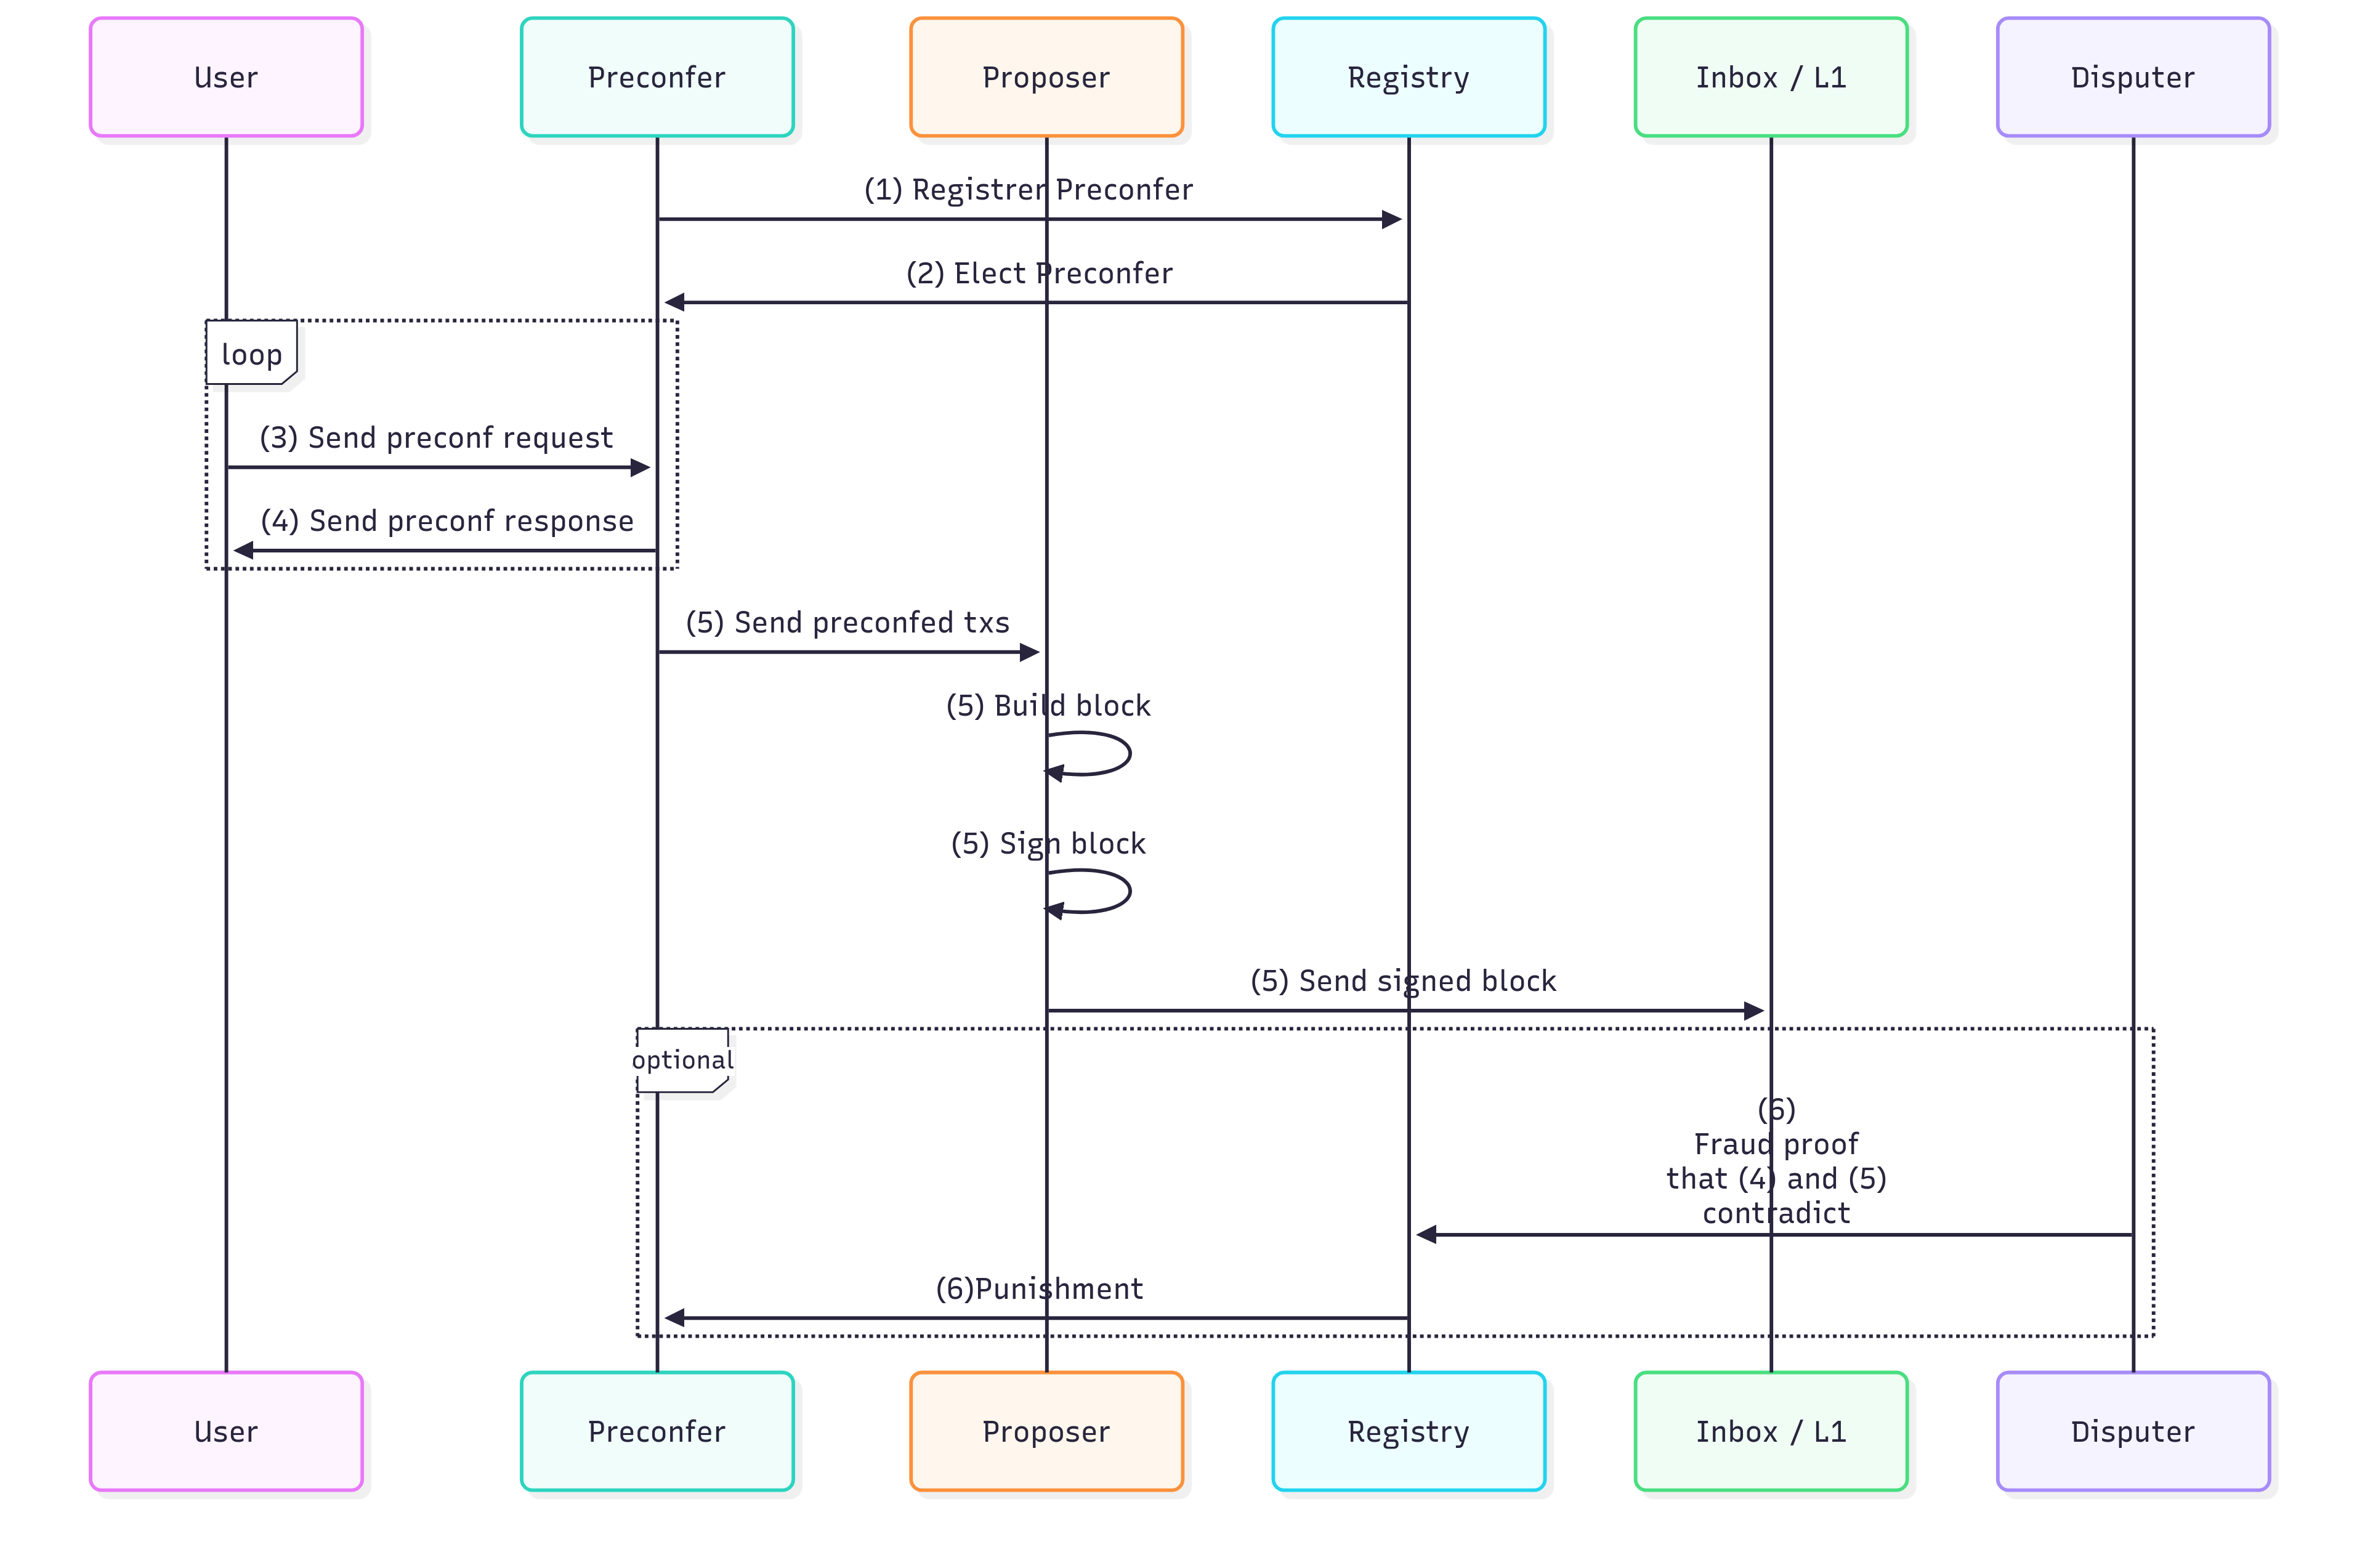
\includegraphics[width=0.9\textwidth]{figures/preconfProtocolFlow.png}
        \caption{Preconf protocol flow.}
        \label{preconf_protocol_flow}
    \end{figure*}
    
\subsection{Step 1: Preconfer registration}
\label{step1:preconfer_registration}
    The first step in our preconf protocol flow is preconfer registration (see Fig.~\ref{preconf_protocol_flow}). Preconfer registration involves candidates signalling that they want to become a preconfer. For this signalling to result in a successful registration, the candidate must satisfy any and all registration conditions including but not limited to:
    \begin{itemize}
        \item Membership of the L1 proposer set
        \item Depositing some minimum slashable collateral.
        \item Governance committee approval
    \end{itemize}

        \subsubsection{Preconfer Registry} \label{preconfer_registry}
        \begin{definition}
        The \textbf{preconfer registry} is a smart contract wherein entities can opt in to preconfing, registering themselves as preconfers. 
        \end{definition}
        For L2 preconfs, a preconfer registry is tightly coupled with the core L2 protocol. If an L2 chooses to enforce preconfs, then the registry will dictate who is allowed to propose blocks~\cite{W:SequencerOpt-InDiscoveryandCommunication}. In contrast, for L1 preconfs, a registry cannot control the proposer set; the L1 proposer election mechanism is unaware of any preconf registry. That being said, L1 preconfer registries are likely still needed, given they enable cryptoeconomic enforcement of certain preconf behaviours. 
 
        Preconfer registries may also store information related to preconfer punishment conditions and mechanisms, as well as managing slashable collateral of registered preconfers. Together, these components can be used to inflict direct monetary punishment on malicious preconfers. A straightforward registry design can directly manage collateral and punishment within the same contract. Other more forward thinking designs have moved to decouple registration from collateral and punishment management in an effort to have a unified ``universal" registry contract \cite{W:UniversalRegistryContract} where individual protocols can customize their slashing requirements outside of the core registry. Although coordination and standardization efforts are required, this type of design has the potential to enable better coordination of proposer election between L2s who delegate proposer election to this unified preconfer registry, more on this in Section \ref{registry_implementations}.
         
        \subsubsection{Slashable collateral}
        \begin{definition}
            In the context of preconfs and specific preconfer, \textbf{slashable collateral} is an amount of tokens that can be slashed in the case of that preconfer's misbehaviour. 
        \end{definition} 
        Any preconfer action that violates the slashing conditions as set out in the registry contract can lead to slashing of the preconfer collateral. Given these conditions reflect the behaviours that are acceptable from a preconfer, the threat of losing some or all slashable collateral as a result of violating a slashing condition acts a deterrent to dishonest preconfer behaviour. Slashing of collateral, and alternative punishment methods are thoroughly discussed in Section~\ref{preconfer_punishment}.  

        \subsubsection{Management of collateral}
        %\lo{would say it is pretty much a requirement rather than "some occasions"} \cm{is the difference trying to be addressed here the ability for the registry contract to slash? In this case, Lin is correct, but Demetris may also be correct in that the collateral may be stored elsewhere e.g. through restaking. Regardless, this needs to be clarified with references.} \dk{I was indeed referring to cases where collateral is stored elsewhere like restaking, it is mentioned in the next sentence but maybe it should be clarified}, 
        
        As mentioned in Section~\ref{preconfer_registry}, registry contracts can directly manage slashable collateral. This requires users to lock up a dedicated collateral to the registry which cannot be reused for other purposes. Therefore, protocols may want to rely on third-party restaking platforms for sourcing slashable collateral, such as the EigenLayer platform~\cite{W:RestakingOverview}. Restaking allows collateral to be reused for multiple purposes, making it an attractive capital-efficient means for sourcing collateral, albeit introducing risks related to stake being slashed in multiple protocols at once. This risk reduces the per-unit security of restaked collateral vs single-use collateral deposited directly to a preconfer registry. For more information on these trade-offs, see \cm{RESTAKING REFERENCE} \lo{The final point is an interesting one, heard some teams wanting ability to have dedicated collateral for their protocol. And IIRC EigenLayer provides this.}.
    

        \subsubsection{Registry implementations} \label{registry_implementations}
        
        At the time of writing, each preconf protocol implements and deploys its own standalone registry contract, such as \cite{W:Documentation-RegisteringasaProvider}.

        However, a different approach has received general support recently, the Universal Registry Contract (URC)~\cite{W:UniversalRegistryContract}. The aim of URC is to create a universal and generic open-source contract that replaces the need to create individual registries and supporting contracts for each preconf protocol. The URC aims to standardise:
         \begin{itemize} 
             \item Preconfer registration.
             \item Preconfer discovery. \lo{"discovery" sounds like finding the RPC endpoint of preconfer, in which URC doesn't help.}
             \item Collateral posting and management.
             \item Restaking integrations with preconf protocols. \lo{URC can support retaking integration, but it doesn't standardize it.}
             \item Slashing and enforcement logic. \lo{URC doesn't standardize slashing logic, just the enforcement part.}
         \end{itemize}

        Lastly, in an attempt to make preconfirming accessible to solo-stakers with limited resources, \cite{W:CrediblyNeutralPreconfirmationCollateral:ThePreconfirmationRegistry} suggests integrating an additional collateral delegation method. Collateral delegation allows the formation of proposer pools and improves capital efficiency for large operators who wish to split their collateral into multiple pools. However, implementing this idea is not straightforward and there are risks and barriers to overcome first. \qb{such as?}

\subsection{Step 2: Preconfer Election}
        Each preconf protocol sets its own preconfer qualification criteria. 
    In addition to registering, a preconfer is required to meet some eligibility criteria before being elected as a preconfer.
        \subsubsection{Eligibility criteria}
        \cm{This section was not focused on eligibility. I've editted but will need further work. Feel free to edit and add} 
        Each protocol has the freedom to set its own eligibility criteria for its preconfers. Generally, preconfers must have the ability to deliver the inclusion / execution of a tx that they issued a preconf for. Some protocols may insist that preconfers be proposers of the underlying blockchain protocol \qb{Thus making them based preconf protocols?}\dk{this sentence should probably go, it is indeed confusing}. Other requirements include the deposit and maintenance of slashable collateral, and non-membership of any preconfer blacklists. 
        % add: Competition is possible (ETs: Spire, Value-capturing based rollups) - delay economics of competition to later section
        \paragraph{collateral}
        \paragraph{lookahead}
        \label{sec:step2_lookahead}

In based preconfs, the preconfer is the next opted‑in L1 proposer listed in the proposer lookahead. The lookahead must therefore be (i) stable and (ii) directly accessible within the EVM, enabling L1 contracts to identify the expected preconfer and, for example, ignore submissions from anyone else.

        \paragraph{whitelist / blacklist}

The preconf protocol can also employ access lists. For example, a whitelist limits preconfers to a trusted set during a “training‑wheels” phase before permissionless launch, or a blacklist that bars entities who violated fair‑exchange guarantees or were previously slashed.

        \subsubsection{Election}
        
        
\subsection{Step 3: Preconf Request} \label{preconf_request}
    As soon as a registered preconfer is elected, users who wish to receive preconfs can begin submitting their signed preconf requests (see Fig.~\ref{preconf_protocol_flow}). Depending on the protocol, users can route their request to the preconfer via P2P~\cite{W:Documentation-Understandingmev-commit} or through RPC endpoints~\cite{W:Towardsanimplementationofbasedpreconfirmationsleveragingrestaking}. The request structure can vary from protocol to protocol. That being said, preconf requests typically include the following:


    

    \begin{itemize}
        \item \textbf{Tx(s)/intent/operation:} Requests are expected to include the tx(s), intent or operation for which the user wishes to receive a preconf. Some protocols have attempted to use preconfs to describe the ahead-of-time commitment to out-source block-building to a specific entity ~\cite{W:Proposer-CommitmentInfrastructureinEthereum}, although these contracts are better known as blockspace deliverables/futures~\cite{W:OpportunitiesandConsiderationsofEthereumsBlockspaceFuture, W:BlockspaceFutures}. We will not consider blockspace futures/deliverables as preconfs in the remainder of this article. Instead we focus only on preconfs where the tx(s), intent, or operation to be included in the block are committed to by the preconfer when responding to a preconf request.
        \tododk{Should we explain intents and operations?}
        % In some protocol designs where preconfs are provided by proposers and blocks are built by builders, users can hide their txs from the builders until they get a preconf~\cite{W:PreconfirmationsundertheNOlens}. 
        
        \item \textbf{Preconf tip:} The preconf tip is compensation to be paid to the preconfer for the preconf. It is atomically binded to the tx so the preconfer cannot redeem the tip without honouring the preconf \lo{Not sure if it has to be atomically bound. For example, you can have non-atomically-bound tip but quick preconfs enforced via fair exchange solution. In a sense, centralized seq can be thought of doing this.}. The tip is the main incentive for preconfers to provide preconfs and therefore it should be properly priced. Preconf tip pricing is handled in detail in Section \ref{EconomicViabilityOfPreconfs}.
        % \cm{finish with something like: pricing is handled in detail in later Section, Section ABC}
        % \cm{for the final document, it doesn't make sense to me to go off topic for the next paragraph and talk about calculating tips. I think this is part of incentives/MEV section which should be later in the doc}
        % However, calculating a sufficient tip is non-trivial and can be very challenging. Preconfers are required to solve an online MEV problem and decide whether to accept or reject a preconf request without having a complete image of all the potential txs they can include in the block. This means that the tip should be alluring enough to make the preconfer commit to including/executing a tx instead of rejecting it for the possibility of increasing MEV later within the slot. Subsequently, the preconfer has a motive to delay responding to requests in order to maximise MEV which leads to the fair-exchange problem that will be further investigated in the next paragraphs~\cite{W:StrawmanningBasedPreconfirmations}. \cm{this comment is referring to what paragraphs? I don't see the logical next here} \qb{agreed}
        
        \item \textbf{Preconf type:} 
        % \cm{why doesn't preconf type need to be specified by all} \qb{I think because the section starts with the idea that the user signs a request that contains some parameters, but the actual type of preconf requested can in some protocols be deduced from the structure of the preconf request itself, hence it doesn't need to be specified (don't recall exactly which article it was, just remember reading it)}
        Provided that the protocol and/or the preconfer support both inclusion and execution preconfs, users might need to specify which type of preconf they want.
    \end{itemize}

    Requests may also contain more nuanced parameters:
    \begin{itemize}
        \item \textbf{Deadline:} A deadline parameter sets the latest possible slot/time before which a request should be considered void, and its tx(s)/intent/operation no longer includable by the preconfer~\cite{W:PreconfirmationsforVanillaBasedRollups}. 
        
        \item \textbf{Tip decay/escalator mechanism:} 
        The preconf tip may need to change during the duration of a request to reflect a request submitter's urgency for a preconf to be fulfilled. A tip decay mechanism decrements the tip that can be redeemed by a preconfer over time. This can incentivise preconfers to respond in a timely fashion~\cite{W:Documentation-BidDecayMechanism}, or reflect some additional value that a transaction provides a preconfer while waiting in the mempool. On the other hand, a tip escalator mechanism increments the tip over time. This incentivises a preconfer to eventually preconfirm a tx~\cite{W:OrderflowauctionsandcentralisationII:orderflowauctions}. Tip escalators are intended to be deployed where preconfers are racing to preconf transactions. This makes tip escalators more appropriate for inclusion preconfs, or execution preconfs with deadlines longer than a singler preconfer's window. \cm{do we use "preconfer window"}
        % Primev use a bid decay mechanism, while fee escalators have also been discussed although not in the context of preconfs \cm{Add fee escalator doc}.  
        
        \item \textbf{Preconf penalty:} Instead of relying on a predetermined penalty system, it is possible that users define preconf penalties for preconfer faults through a request parameter~\cite{W:User-DefinedPenalties:EnsuringHonestPreconfBehavior, W:Documentation-BidStructure}. The idea is to allow users and preconfers to mutually agree on a level of crypto-economic security where a ``one-size-fits-all" approach does not suffice.
        
        \item \textbf{Latest blockchain state:} 
        It is possible for protocols to allow users to specify the state root hash of the current blockchain state in their request~\cite{W:AnalyzingBFTProposer-PromisedPreconfirmations}. This gives users control over what state their request acts on.
        
        \item \textbf{Privacy preferences:} 
        Privacy-preserving techniques may be applied to preconf requests to hide key request data from unwanted entities in the block-building pipeline \qb{are there "unwanted entities" in the pipe-line? perhaps untrusted fits better?}, including some subset of preconfers, or even from preconfers themselves until a response is provided. Techniques include public-key encryption, or trusted intermediaries as are used in MEV-Boost works today~\cite{W:BasedPreconfirmationswithMulti-roundMEV-Boost, W:AnalyzingBFTProposer-PromisedPreconfirmations, W:Documentation-BidStructure, W:Towardsanimplementationofbasedpreconfirmationsleveragingrestaking}.
         
    \end{itemize}
    
    
\subsection{Step 4: Preconf Response} \label{preconf_response}
        
    After observing a preconf request and verifying its validity, the preconfer must then choose whether to provide a preconf or not. This section describes the process of responding to preconf requests. Generally, preconfers should be incentivised by the protocol to provide timely responses to users in order to improve UX. Incentivising timely preconf responses is discussed in detail in Section \ref{fair_exchange_problem}. 
    
    % \cm{following paragraph needs to be clearly and precisely rewritten} A preconf response accepting a request is essentially a preconfirmation (preconf), i.e. a commitment by the preconfer to include/execute a tx. Additionally, rejections do not necessarily constrain preconfers from including the tx in the block unless they are specified by the protocol as non-commitments. Non-commitments are slashable commitments by preconfers to not include the tx~\cite{W:SolutionstothePreconfFairExchangeProblem}. 
    
    Accepting a preconf request binds the preconfer to a commitment to include or execute the preconfirmed tx/intent/operation. In many protocols, preconf responses double up as evidence for punishing dishonest preconfers that fail to deliver a preconf as responded to. Typically, a preconf response is signed by the preconfer and it includes:

    \todocm{ensure standardised preconf responses are discussed in the context of the universal registry. It may be more appropriate to state this once in the URC section}

    \begin{itemize}
        \item \textbf{Unique identifier to a preconf request:}
        A response must contain a unique mapping to the request it is directed at. A hash of a signed request is such a mapping~\cite{W:Documentation-Commitments}.
        
        \item \textbf{Block number containing the requested tx/intent/operation:} Some preconf protocols may require the preconfer to disclose the number of the block that will contain the requested tx/intent/operation~\cite{W:Towardsanimplementationofbasedpreconfirmationsleveragingrestaking}.

        \item \textbf{Updated blockchain state} For execution preconfs, the preconfer may be required to provide a reference to the updated blockchain state at the instant when the preconf response was provided~\cite{W:AnalyzingBFTProposer-PromisedPreconfirmations}. Such a reference can take the form of and updated state root before/after the transaction in the response was executed, or simply the stream of transactions executed up to and including the response.
        
        \item \textbf{More parameters?}
    \end{itemize}
    

\subsubsection{Fair-Exchange of Preconf Requests and Responses} \label{fair_exchange_problem}
    Equally important to the core concepts of requests and responses is the fair exchange of requests and responses. 
    \begin{definition}
        
    The \textbf{fair exchange problem} states that during a mutual exchange of items between two parties, it is vital to guarantee that both parties or neither party receive the expected item. No party should have the ability to gain an advantage by misbehaving or quitting the transaction prematurely~\cite{P:Fairexchangewithasemi-trustedthirdparty}.
    \end{definition}

    In the context of preconfs, users should have some expectation of how and when responses are received after submitting a request. This expectation depends on many factors, including but not limited to the type of preconf, the tip being paid, the cost to provide and deliver the preconf, the relative demand for txs/preconfs at the time the request was sent, and the value that a preconfer can extract from the preconf beyond the tip. Crucially, a preconf user's expectation has a time component built in, i.e. users typically want preconfs sooner rather than later. This makes the fair exchange of preconfs more complex than eventual fair exchange of request and response. \cite{W:PreconfirmationFairExchange} introduces this problem of timely fair exchange, specifically focusing on its presence in preconf protocols. Previous work on fair exchange proved that it is impossible to enforce fair-exchange without an overseer to identify preconfer faults~\cite{P:OntheImpossibilityofFairExchangewithoutaTrustedThirdParty}.
    
    \begin{definition}
    In the context of preconf procotols, an \textbf{overseer} is an entity or set of entities that is trusted to observe the actions of preconfers, and provide signals to the protocol in the case of a preconfer's deviation from protocol rules or expected actions. These signals can include proofs of deviation, although some deviations may not be provable, depending instead on overseer trust. Overseer signals may be communicated on-chain through protocol smart contracts, or off-chain through P2P communication layers. \qb{we generally use P2P network, so I think we should standardize} 
    \end{definition}

    Several overseer election mechanisms have been discussed. The primary distinction of these protocols is based on whether the overseer can signal preconfer misbehaviour in-protocol or not. In-protocol signalling allows for explicit preconfer punishment, something which is discussed in Section \ref{preconfer_punishment}. Such overseers can be elected by governance, or be required to hold some large amount blockchain's native token for which the preconfs are being provided. Both of these preconfer election mechanisms align overseers with the success and reliability of the preconf protocol. 
    
    For overseers who are expected to signal preconfer deviation out-of-protocol, several solutions have been discussed to date. In \cite{W:PreconfirmationFairExchange}, users are collectively identified as a suitable overseer in certain preconf protocols. Users can use the threat of withholding orderflow from a misbehaving preconfer to incentivize preconfers to follow protocol rules. The effectiveness of orderflow withholding as a threat is greatest when there is a single preconfer for the duration of the protocol, as in single-proposer L2s. For every additional preconfer added to the preconfer set, the effectiveness of orderflow loss is diminished proportionally to the number of preconfers; if a preconfer only has access to orderflow once every $N$ slots in expectation, the threat of orderflow loss for that preconfer is $1/N$th of the threat of the single preconfer case. As such, if possible, elected overseers should be favoured over users to enforce timely fair exchange of preconfs with a large/permissionless set of preconfers. 
    
    Wallet providers operating as out-of-protocol overseers on behalf of users is also discussed in \cite{W:PreconfirmationFairExchange}. As wallet providers are more sophisticated than a typical blockchain user, wallets providers may be better suited to identify preconfer deviations.
    In a similar vein, \cite{W:ThePreconfirmationGatewayUnlockingPreconfirmations:FromUsertoPreconfer} presents the concept of gateways or relays acting as overseers on behalf of users by monitoring preconfer behavior and withholding requests or tips. However, as gateways and relays are also being considered as preconf provider \cm{verify relays distinct from gateways in preconf section} preconfs~\cite{W:ThePreconfirmationGatewayUnlockingPreconfirmations:FromUsertoPreconfer}, alternative overseer solutions must also be considered. 
    
    

    
    
    \cm{The following are specific issues related to pricing/ implementation/ preconfing that should be elsewhere}

    

    
    \cite{W:BasedPreconfirmationswithMulti-roundMEV-Boost} proposed splitting each slot into a fixed number of rounds and performing multiple MEV-boost auctions. Each round creates partial blocks that are combined into a single block at the end of the slot. Among other benefits put forward by that proposal, it is argued that multi-round MEV-boost auctions will simplify tip pricing and mitigate the fair-exchange problem.
    
\subsection{Step 5: Delivery/Publication of Preconf} \label{preconf_delivery}

\dk{need to link proposer and preconfer to comply with the diagram}

\begin{itemize}
    \item gateway delivery vs proposer delivery
    \item based vs non-based preconf
\end{itemize}
    
\subsection{Step 6: Preconfer Punishment} \label{preconfer_punishment}    
    Once a preconf is delivered and published, it needs to be verified that the preconfed tx(s)/intent/operation \dk{maybe we need a name for "tx(s)/intent/operation" to avoid writting the whole thing over and over again} \cm{maybe request is appropriate? We can make this connection in the request section if so.} was included or executed as specified by the preconf request and response. Punishments can be utilized to ensure preconfers deliver preconfs according to any restrictions set out in the request or response.
    
    \subsubsection{Preconfer faults and punishing conditions} \label{preconfer_faults_and_punishing_conditions}
    There are various faults that a malicious or negligent preconfer can commit and can jeopardise the smooth operation of a preconf protocol. Fig.~\ref{preconfer fault tree} presents a decision tree that categorises preconf faults.
    \begin{definition}
        The \textbf{punishing conditions} is a list of faults that preconfers should avoid committing otherwise they can be susceptible to punishment. They are put in place to act as a disincentive to malicious preconfer behaviour.
    \end{definition}

\vspace{5mm}
    Preconfer faults are as follows:

    \paragraph{Safety fault}
        \begin{definition}
            A \textbf{safety fault} occurs when the preconfer has published a block without including a preconfirmed tx/intent/operation. 
        \end{definition}
        
        Committing a safety fault is a strong indication of malicious preconfer behaviour. It is a serious fault that should never happen and the punishment is expected to be severe~\cite{W:Basedpreconfirmations}.
        
    \paragraph{Liveness fault}
    \todolo{Add definition nuance regarding missing slot for based L2 vs others}
        \begin{definition}
            A \textbf{liveness fault} occurs when the preconfer misses the slot,  does not publish a block, and therefore the preconf tx(s)/intent/operation is not included on-chain. 
        \end{definition}
        
        A liveness fault could potentially be accidental and non-malicious, for example, due to a power outage or internet downtime. Therefore, protocols may want a lighter punishment for liveness faults. That being said, liveness faults can be indistinguishable from safety faults and may need to be punished severely~\cite{W:Basedpreconfirmations} \cm{this is a bold statement, so we need an example if this is true.}. To mitigate the punishments needed in the case of an accidental liveness fault, \cite{W:AvoidingAccidentalLivenessFaultsforBasedPreconfs} suggests a chained preconf system where following preconfers in the lookahead can honour a preconf that was not fulfilled by the active preconfer due to liveness failure. \cm{Introducing a protocol like this requires 1 or 2 more sentences so the SOK is self-contained. Why would the following preconfer chain preconfs? Any limitations to this chaining protocol?}
        

    \paragraph{Condition Fault \dk{or Broken request conditions or parametric fault or Specification Fault or Constraint Fault}}
        \begin{definition}
            A \textbf{condition fault} occurs when a preconfirmed tx/intent/operation is included on-chain but the preconfer fails to comply with the conditions specified in the preconf request and agreed upon in the preconf response.
        \end{definition}
            
        As explained in section \ref{preconf_request}, users can set various parameters in their preconf request. If the preconfirmed tx(s)/intent/operation is included or executed, but without complying with the conditions set by the user, the preconfer should be liable to punishment~\cite{W:DelegationinBolt:OutsourcingSophisticationWhilePreservingDecentralization}.
        
    \paragraph{Idleness fault}
        \begin{definition}
            An \textbf{idleness fault} occurs when a preconfer receives valid preconf requests but neglects their duty and fails to provide preconf services.
        \end{definition}
       Idleness faults have not been well-documented, but it is natural for some preconf protocols to insist that preconfers provide preconfs under certain conditions, such as:
        \begin{itemize}
            \item Preconfing all requests
            \item Preconfing all requests that do not conflict with an already preconfed and/or confirmed transaction.
            \item Preconfing all requests paying tips greater than a certain amount
            \item Preconfing all requests if and only if there exists a batch of requests paying tips greater than some minimum total amount. 
            
        \end{itemize}
        As idleness faults depend on requests being delivered to the preconfer but not being responded to, this introduces a subjective observability requirement for the overseer.
        
        As illustrated in sections \ref{preconf_response} and \ref{EconomicViabilityOfPreconfs} \dk{this should be adjusted to point to preconf pricing}, there are various factors that can influence a preconfer's decision to provide a preconf, such as the preconf tip and the incompatibility of conflicting txs. Therefore, idleness faults can be handled by an overseer \cm{if not handled by an overseer, who else can handle this? Personally, I think we can say something stronger "likely need to be handled"}.

    \begin{figure}[htbp]
        \centering
        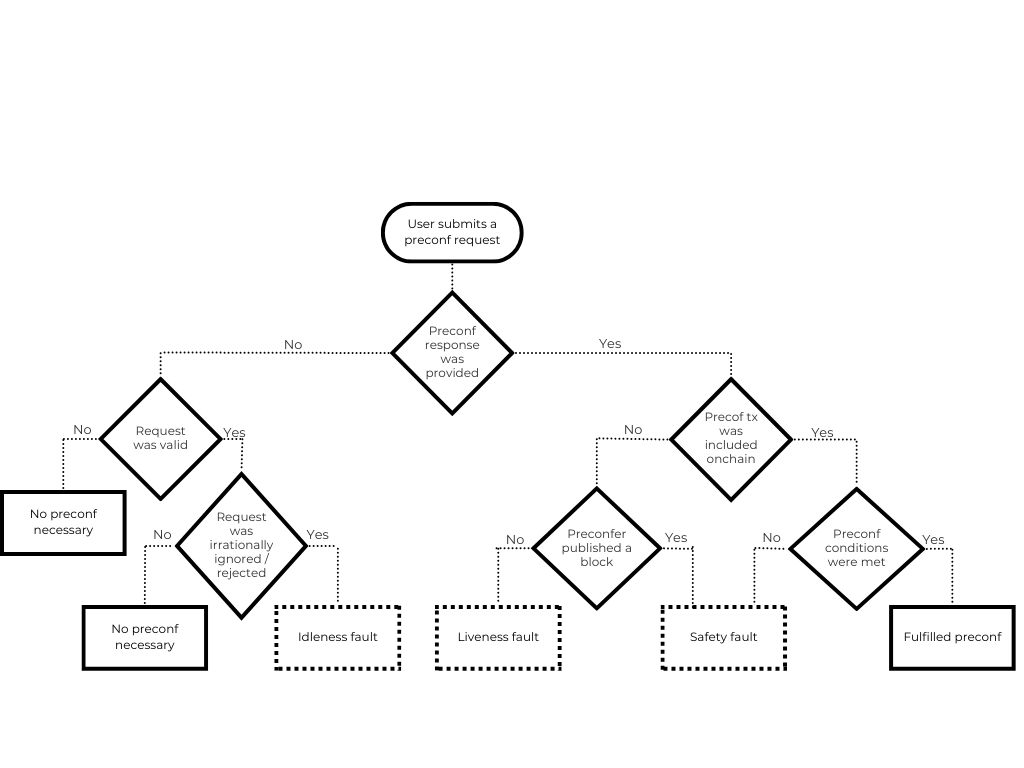
\includegraphics[width=0.9\textwidth]{figures/preconferFaultDecisionTree.png}
        \caption{Preconfer fault decision tree.}
        \label{preconfer fault tree}
    \end{figure}
    

\subsubsection{Enforcement Mechanisms (EM) and proofs of malicious baheviour} 
    Preconf protocols rely on economic incentives to encourage honest preconfer behaviour. However, relying solely on incentives may not be sufficient. Therefore, protocols incorporate mechanisms to punish malicious preconfer behaviour.

    \begin{definition}
        An \textbf{enforcement mechanism} (EM) is a mechanism 
        triggered when a preconfer violates a punishing condition. The EM initiates the punishment of the malicious preconfer.
    \end{definition}

    Although the main idea of an EM is the same, there are different approaches. The key differences between them are whether they are permissionless or permissioned, the type of proof they require to be triggered, and the type of enforcement~\cite{W:PreconfirmationFairExchange}.

    In a permissioned setting, punishment through the EM is initiated by a member of an overseer committee. The committee is composed of trusted and whitelisted entities explicitly designated by the protocol. Generally, the proofs required to initiate punishment in this environment are less rigorous.  As long as the committee reaches consensus that a dishonest preconfer should punished, EM can be triggered without further proof. Naturally, this could raise concerns about centralisation, censorship or liveness~\cite{W:PreconfirmationFairExchange}.

    In a permissionless setting, anyone can act as an overseer to initiate punishment via EM and there are economic incentives to for users to do so. Contrary to a permissioned environment, in this environment, the overseer is required to submit conclusive and indisputable evidence to back up the claim of malicious preconfer behaviour. The main evidence that can be used to prove malicious behaviour are the signed preconf request and response which are checked against the published blocks. Any accused preconfer who fails to submit evidence against the claim is exposed to punishment~\cite{W:GitHub-UniversalRegistryContract,W:GitHub-ExampleSlasherImplementations,W:PreconfirmationFairExchange}.

    \subsubsection{Punishments}
    
    Preconfer punishments are intended to result in economic consequences. These consequences can be direct or indirect. Direct preconfer punishments involve collateral slashing. Indirect preconfer punishments target preconfer's profit from preconfs~\cite{W:PreconfirmationFairExchange}. 
    
    Punishments can also be divided into real-time or ex-post depending on when they are enforced. In real-time punishment, preconfer's actions are closely monitored by an overseer and any misbehaviour is immediately detected preventing preconfer from making any profit. As a result, this system requires overseer liveness to operate. 
    
    Ex-post punishments penalise dishonest preconfers retrospectively. Slashing is the most direct and straighforward ex-post punishment. If any of the slashing conditions is violated, the preconfer loses a predetermined amount of their collateral. Moreover, a preconfer can be temporarily blacklisted, i.e. be deprived of their right to provide preconfs or have their stake temporarily frozen. Other than that, the protocol can limit the preconf orderflow of dishonest preconfers or downgrade their reputation to affect future orderflow~\cite{W:PreconfirmationFairExchange,W:User-DefinedPenalties:EnsuringHonestPreconfBehavior}.




\section*{Preconf Economics}
Preconfs require proposers to commit to blockspace earlier than proposal time. This is problematic for proposers, as blockspace potentially becomes more profitable if assigned at the last possible instant before proposal time. Without enforcement or explicit payments, preconfers have an incentive to withhold preconf responses as late as possible. By doing so, preconfers act on up-to-date information, while increasing the number of transactions in the mempool, and the number of possible transaction orderings. All of these things contribute to a preconfer's ability to extract MEV from the mempool \cite{W:AnalyzingBFTProposer-PromisedPreconfirmations,W:StrawmanningBasedPreconfirmations}. In contract, user demand for preconfs translates to users having utility to receive a confirmation of transaction execution or inclusion before a proposer proposes a block for consensus, with this utility decreasing in time after a request is sent. \cm{check wording of this sentence is consistent}.

    To address the tension of users wanting preconf responses quickly, and proposers wanting to wait as long as possible before a response is provided, proposer incentives are needed. We have already seen in Section~\ref{preconfer_punishment} that the preconfer role can be subjected to punishment conditions to incentivize certain behaviours, including timely responses to requests. Just as punishments can be applied for slow responses, rewards in the form of preconf tips can be applied for timely responses. 

    This \cm{chapter?}/section focuses on preconf economics, with particular focus on how the revenue of proposers changes under preconfs, how preconfs are priced, how preconfs are economically enforced, and the economic risks that preconfs pose to the key stakeholders in the block-building pipeline
\section{Impact of Preconfs on Proposer Revenue}
    
     Several works have attempted to model expected proposer revenue from preconfs\cite{W:PreconfirmationsundertheNOlens,W:EstimatingtheRevenuefromIndependentSub-SlotAuctionPreconfirmations,W:AnalysingExpectedProposerRevenuefromPreconfirmations,W:APricingModelforInclusionPreconfirmations} \todocm{identify other pricing works}. There are two key takeaways from these works.
     
     \begin{enumerate}
         \item Inclusion preconfs are a straightforward way for proposers to increase their revenue without disrupting their expected revenue from existing block-building strategies, MEV-Boost, commit boost, or otherwise \cite{W:APricingModelforInclusionPreconfirmations}.
         \item Execution preconfs require preconfer sophistication and/or significant preconf-specific tip revenue to make execution preconfs economically viable for proposers with the option not to preconf \cite{W:PreconfirmationsundertheNOlens,W:EstimatingtheRevenuefromIndependentSub-SlotAuctionPreconfirmations,W:AnalysingExpectedProposerRevenuefromPreconfirmations}. 
     \end{enumerate}
    
    \subsection{Inclusion Preconfs \& Proposer Revenue}

    \todocm{Key Takeaways from incl. preconf work}
    Inclusion preconfs provide proposers with a new source of txs and tx revenue that is expected to increase proposer revenues without the need for proposer sophistication. This result is presented in \cite{W:APricingModelforInclusionPreconfirmations}. In this article, the author's show that thanks to the flexibility that inclusion preconfs give proposers with respect to where preconfed txs can be included in a block, proposers can price inclusion preconfs using basic pricing models. More than this, proposers can sell significant amounts of block-space through inclusion preconfs without interfering with expected block-building revenues. 
    
    The article identifies that block-space, measured in Eth per gas, is most valuable at the start of Ethereum blocks, and least valuable at the end of blocks. Specifically, cumulative tx fees in block-space follow a lognormal distribution. This aligns with results from MEV literature that has formally proven that early access to DEX state has significant value for sophisticated MEV extractor \todocm{LVR reference}. As inclusion preconfs need only compete for the least valuable block-space, inclusion preconfs can be priced in the same way as this least valuable block-space. Given the logarithmic nature of cumulative tx fees vs. block-space, basic price curves can be utilized by proposers to price inclusion preconfs for the first $X$\% of block-space, for any $X$ that avoids contention with the highest MEV parts of a block. 
    
    Critically, proposers offering inclusion preconfs can always reject preconfs, and utilize existing block-building methods at proposal time, such as MEV-Boost. Inclusion preconfs therefore stand as an easy-to-price add-on for proposers that can be offered with negligible probability of decreasing revenue. Of course, pricing sophistication is always possible. Although conservative inclusion preconf pricing can be employed to ensure proposer revenues do not decrease, proposers can increase expected revenues by offering prices in-line with preconf demand, up-to-date estimates of block-building revenues, as well as granular per-unit block-space pricing models. 

    \subsection{Execution Preconfs \& Proposer Revenue}
    \todocm{settle on storyline}
    \begin{enumerate}
        \item ISSAs vs DSSAs
        \item ISSAs reduce revenue without tips
        \item DSSAs increase revenue, but require preconfer sophistication. 
        \item Where does chorus one article fit in?
    \end{enumerate}
    

    % LEGO 1
    Meanwhile, an analysis by Nethermind \cite{W:EstimatingtheRevenuefromIndependentSub-SlotAuctionPreconfirmations} estimates that proposer's revenue will be significantly reduced with the introduction of independent sub-slot auctions (ISSAs) to facilitate execution preconfs.
        
    ISSAs is a proposal aligned with Multi-round MEV-Boost~\cite{W:BasedPreconfirmationswithMulti-roundMEV-Boost} and suggests splitting slots into rounds of equal length. For each round the proposer holds an independent auction to build sub-blocks which are then combined into a block.

    To perform the impact analysis, the components of proposer's profit were classified into categories. It was then forecasted that for most components the reward decays exponentially as the number of rounds per slot as the number of rounds increases. Overall, it was estimated that 8 rounds can reduce proposer's rewards by 50\% while continuous preconfs (assuming unlimited rounds) can reduce proposer's revenue by 74\% compared to the conventional end-of-slot MEV-Boost auction.

    This result emphasises the importance of preconf tips as compensation for proposers. Additionally, it suggests that, in order to be viable, preconfs should be priced to at least match the proposers' loss from providing them. This could also be a first step towards answering question \textbf{\ref{Q_pricing}} about preconf pricing.
    
    % LEGO 2
    Further research by the same team presents the theoretical concept of dependent sub-slot auctions (DSSAs) for facilitating execution preconfs~\cite{W:AnalysingExpectedProposerRevenuefromPreconfirmations}. According to the analysis, DSSAs can increase proposer's expected revenue compared to MEV-boost even without preconf tips.

    Similarly to ISSAs, there is an auction for every sub-slot the winner of which has the right to build the sub-block of the sub-slot. The main difference between ISSAs and DSSAs is that the auction winner also becomes the \textit{active proposer}. The active proposer is the entity with the right to build the remaining of the Ethereum block, thus entitled to the expected revenue of the rest of the block. The first active proposer of each slot is appointed as defined in the lookahead and is responsible to bundle the sub-blocks together in a block at the end of the slot.

    Overall, the active proposer at any sub-slot has the right to build the sub-block or auction off the position of the active proposer for an amount that is at least as much as the expected revenue for the remainder of the slot. The active proposer can also decide whether to offer preconfs to further increase revenue from preconf tips.

    In \cite{W:PreconfirmationsundertheNOlens} addresses about the impact of preconfs on proposer and searcher rewards in the current PBS setup. It is projected that proposers could increase their revenues at searchers' expense. On the other hand, searchers will need to adapt their bidding behaviour and employ more sophisticated bidding strategies. With the introduction of preconfs, searchers can no longer rely on private communication with builders who have a probability of winning an auction to build a block. This happens because searchers will be able to receive execution preconf for a transaction directly by the proposer. Therefore, searchers are expected to start biding earlier and more aggressively to have their txs preconfirmed.
    
    \subsection{Preconf Pricing}

     
    
\subsection{Economic viability of preconfs} 
\label{EconomicViabilityOfPreconfs}
    

 
    % Preconfirmations under the NO lens
    

    % LEGO 3
    In contrast to execution preconfs, for inclusion preconfs, proposer's expected profit from offering inclusion preconfs is greater than not offering them~\cite{W:AnalysingExpectedProposerRevenuefromPreconfirmations}. Furthermore, although there is no established pricing method, multiple formal models for pricing inclusion preconfs have been put forward~\cite{W:APricingModelforInclusionPreconfirmations,W:PricingTransactionsforPreconfirmation}.

    

    % Pricing Transactions for Preconfirmation
    A different pricing model was presented by a Chorus One research team~\cite{W:PricingTransactionsforPreconfirmation}. This model agrees that txs should be preconfirmed only if they compensate for inclusion risk and produce expected revenue that is equal or greater than MEV-boost. However, the model follows a slightly alternative approach as it suggests using mid-block txs to price inclusion preconfs. Additionally, instead of explicitly pricing inclusion preconfs, it calculates a threshold expressing priority fee per unit of gas that a tx should have to be preconfirmed.

    Initially, the team categorised txs into three tiers based on their position in the block and demonstrated that, on average, the higher the position, the higher the builder's priority fee per unit of gas. Then, data from tiers 1 and 3 were excluded before training three different models (heuristic-based, linear regression, and random forest) that predict the threshold. Tier 1 data were excluded to reduce bias from private order-flow and MEV txs with high priority fees, tier 3 data were excluded to reduce bias from late tx arrival pricing premium.

    After evaluating the models, it was concluded that the random forest model seems to outperform the other two as it can capture more complex data relationships. Also, the results reveal a clear tradeoff as lower threshold means that more txs are preconfirmed, but the loss from incorrectly priced or unprofitable preconfs is higher.

    Overall, concerning question \textbf{\ref{Q_diffs_inc_exec}} preliminary results of preconf viability research seem to converge to the conclusion that without preconf tips, execution preconfs are generally expected to decrease proposer's expected profit while inclusion preconfs are expected to increase it. Moreover, pricing inclusion preconfs is significantly easier and there is no effective method to price execution preconfs yet.

    % Value-capturing based rollups with based preconfirmations
    For question \textbf{\ref{Q_based_seq_profit}}, current based rollups are designed so that all revenue is captured by the L1 proposer who controls sequencing. \cite{W:Value-CapturingBasedRollupswithBasedPreconfirmations} suggests a new protocol design that enables rollups to capture some value.

    According to the proposal, L1 proposers will be charged for sequencing rights in the form of an auction. Auction's profits will be absorbed by the rollup. Once the lookup of an epoch is known, each proposer of a slot i can bid to gain preconfer rights for a series of consecutive slots ending in slot i. The winner of the auction of each slot inherits the right to interact with rollup's smart contract to propose a new based rollup block. Owning sequencing rights for consecutive blocks can be more profitable than owning rights for two separate blocks which gives incentive to proposers to bid in the auction. Furthermore, L1 sequencers can increase their revenue by providing preconfs.

    As for question \textbf{\ref{Q_quantify_benefits}}, accurately quantifying the benefits and the value of UX improvement remains a challenge. Undoubtedly, enhancing UX improves the protocol and increases user utility and demand. At the same time, preconfs decrease MEV. Computing MEV loss is relatively simple, but calculating the value of increasing utility and demand and estimating a fair price that users would agree to pay for preconfs is still puzzling, especially without relevant data. It is possible that preconf protocols would need to go through a pilot phase of experimentation and data gathering which before they can properly answer this question.

    \section{Risks \& Considerations} % \section{Additional implications/changes/effects}
    In this section, we focus on risks and considerations that can influence design and implementation choices of a preconf protocol. They are split into different categories according to the entity that could be the most affected by them. It is essential to note that this is not an exhaustive list as novel risks and considerations may emerge, for example, with the introduction of new EIPs for Ethereum~\cite{W:Future-ProofingPreconfirmations}. Furthermore, the economic viability of preconf protocols is a major consideration, but it will not be analysed further since it was already covered in depth in Section \dk{add reference to the Economics section}.

    \subsection{for the ecosystem \dk{or everybody/systemic}}

    \begin{itemize}
        \item \textbf{Smart contract risk:} Similarly to every Web3 protocol that is controlled by smart contracts, preconfs can be prone to smart contract risk, i.e. code errors and vulnerabilities~\cite{W:SmartContractVulnerabilitiesandMitigationStrategies}. The risk could be amplified because the concept of preconfs is recent, complicated and has not been thoroughly battle-tested yet. To mitigate risk, smart contracts must be extensively audited to ensure that they are trustworthy before they are deployed~\cite{W:CrediblyNeutralPreconfirmationCollateral:ThePreconfirmationRegistry}. Another potential idea would be the creation of a competitive environment between different preconf protocols and between preconfer as proposed in \cite{W:ThePreconfirmationSauna}. Such an environment encourages a repeated game from which existing protocols will be improved and new protocols will emerge.
        
        \item \textbf{Centralisation problem:} Inevitably, any implementation of preconfs will require a certain level of additional sophistication. As a result, preconfers may choose to outsource technical expertise by delegating preconf duties to gateways. The more complicated the protocol becomes, the less participants will be able to follow and less entities will be entrusted with preconfer duties. This could pose a major centralisation risk for the whole ecosystem~\cite{W:DelegationinBolt:OutsourcingSophisticationWhilePreservingDecentralization,W:BecomingBased:APathtowardsDecentralisedSequencing}.\dk{should we also talk about overseers here?}
    
        \item \textbf{Liveness:}
        Implementations that grant exclusive preconfer rights to a single entity in each slot might be exposed to liveness risk. Granting complete control creates a single point of failure and raises censorship concerns for the duration of the slot~\cite{W:StrawmanningBasedPreconfirmations,W:BasedPreconfirmationswithMulti-roundMEV-Boost}. 
        % This is an issue with "streaming" continuous preconfs. 
        
        \item \textbf{Latency races:} 
        Users could potentially benefit from having the lowest latency to the preconfers in protocols that offer continuous preconfs\dk{the term continuous preconfs should be explained, maybe in the economics section}. Minimum latency can maximise MEV back-running profit as users with the lowest latency can have priority to accessing the latest chain state and submitting back-run txs. Besides creating inequalities among users, latency races can also lead to geographical centralisation~\cite{W:StrawmanningBasedPreconfirmations}. 
        Single-proposer protocols are more exposed to this risk as the location of the preconfer remains constant. A potential solution could be batching preconfs in subslots instead of proving them continuously~\cite{W:BasedPreconfirmationswithMulti-roundMEV-Boost}.
                
        \item \textbf{Congestion:} 
        Protocols that support continuous preconfs may also be vulnerable to congestion risk. Especially in L2s where gas fees are lower, users can spam the network with probabilistic arbitrage attempts. Congestion increases gas prices as a result of increased demand for block space. At the same time, block space is wasted in failed arbitrage txs. The congestion risk could be mitigated with an auction-based system that encourages users to participate in a bidding contest instead of flooding the network~\cite{W:StrawmanningBasedPreconfirmations,W:BasedPreconfirmationswithMulti-roundMEV-Boost}.
    
    \end{itemize}

    \subsection{for preconfers}
    \begin{itemize}
        \item \textbf{Slashing:}
        Preconfers are required to opt-in to punishing conditions, including slashing conditions, and lock up a slashable collateral. Slashing is probably the main risk that preconfers take on. Slashing conditions act as a safeguard designed to deter malicious behaviour. However, as explained in section \ref{preconfer_faults_and_punishing_conditions}, even honest preconfers may be vulnerable to accidental liveness slashing~\cite{W:AvoidingAccidentalLivenessFaultsforBasedPreconfs}.

        
        \item \textbf{Sophistication requirements:} 
        Preconf protocols are bound to have some sophistication requirements from the preconfers. The complexity requirements, paired with any implicitly necessary capital requirements, should be a serious consideration for potential preconfers. Meanwhile, builders already have the infrastructure and experience to take on additional expertise. Consequently, proposers may be tempted to delegate their preconf duties to builders which, if left uncontrolled, can lead to the aforementioned centralisation problem~\cite{W:Towardsanimplementationofbasedpreconfirmationsleveragingrestaking,W:AnalysingExpectedProposerRevenuefromPreconfirmations}.
        
        \item \textbf{Fault attribution:}
        When all preconfer duties are performed by a single entity in each slot, fault attribution is relatively straightforward in case of punishing condition violation. Nonetheless, attribution becomes significantly more convoluted when duties are delegated or distributed~\cite{W:DelegationinBolt:OutsourcingSophisticationWhilePreservingDecentralization}. Protocols that support the separation of the preconf pipeline among multiple independent entities should carefully design mechanisms to ensure that fault attribution remains as transparent and objective as possible.
        
        \item \textbf{Legal risk:} 
        The legal risk associated with preconfs is not widely discussed. However, the structure of a preconf shares common characteristics with a formal agreement, raising the question of whether a preconf could constitute a legally binding contract. If so, violating the protocol's punishing conditions could potentially carry legal consequences for the preconfer. To mitigate this risk, protocols may need to consider including explicit disclaimers to limit the legal liability of preconfers.

    \end{itemize}
    
    \subsection{for users}

    \begin{itemize}
        \item \textbf{Increased gas prices:} 
        % potential implication / collateral effect
        % may affect all users and not just the ones requesting preconfs
        % Making preconfs attractive to proposers probably requires increasing gas fees. 
        % Also increased demand from improved UX can drive gas prices up
        
        \item \textbf{Sophisticated user requirement:} % requesting a preconf entails some additional sophistication, most sophistication could be hidden behind the wallet (Analysing Expected Proposer Revenue from Preconfirmations)
        
        \item \textbf{Frontrun hazard for non-preconfirmed txs:} %preconfs may bring a requirement for everyone to use preconfs, which may be worse UX for some users. Can we have preconfs which are "at least as easy to use as current transactions?"  if everyone is doing preconfs and you don't, you might be in a bad position (Analyzing BFT & Proposer-Promised Preconfirmations)
        
        \item \textbf{Deposit requirement:} 
        % certain protocol desings
        %requirement to maintain funds in multiple platforrms, depends on the design (not standard) some protocols require users to post a collateral (Proposer-Commitment Infrastructure in Ethereum)
    \end{itemize}
    
    \subsection{for L1 scaling solutions (LNs)}
    \begin{itemize}
        \item \textbf{Increased delay on transaction execution:} % not every L1 proposer has opted-in to give preconfs (Analyzing BFT & Proposer-Promised Preconfirmations)
        
        \item \textbf{Fallback based preconfer needs to be implemented correctly:} % Mechanism that ensures liveness by reassigning preconfer rights when there is no active preconfer. This happends when there are no based preconfers left in current epoch or the current preconfers are not responding. (Sequencer Opt-In, Discovery and Communication, Becoming Based: A Path towards Decentralised Sequencing)
        
        \item \textbf{Trade-off between centralised and decentralised sequencing:} % centralised: high thoughput, low latency, easy preconfs but it has centralisation, censorship, liveness hazards and trust requirements. Widely adopted based rollups with preconfs can achieve high performance (Becoming Based: A Path towards Decentralised Sequencing)
    \end{itemize}


\section{Implementations \& existing protocols}

        \subsubsection{ \textbf{Primev's MEV-commit}}
        % https://docs.primev.xyz/v1.1.0/get-started/welcome-to-primev
        % https://docs.primev.xyz/v1.1.0/concepts/rewards-and-slashing/rewards-and-slashing
        % https://ethresear.ch/t/preconfirmation-fair-exchange/21891
        

        \subsubsection{ \textbf{Chainbound's Bolt}}
        % https://research.chainbound.io/
        % https://research.chainbound.io/delegation-in-bolt-outsourcing-sophistication-while-preserving-decentralization
        % https://research.lido.fi/t/proposal-onboard-bolt-to-the-lido-alliance/7724/2
        % https://research.chainbound.io/examining-the-based-sequencing-spectrum
        % https://research.chainbound.io/exploring-verifiable-continuous-sequencing-with-delay-functions
        
        \subsubsection{ \textbf{Taiko with Nethermind's enforcement mechanism}}
        % https://taiko.mirror.xyz/ejciROGOGM9L_DuuqM3KloZan0EQR73fJt8qzTZmVzg
        % https://4pillars.io/en/articles/preconfirmation-feat-taiko
        % https://en.theblockbeats.news/news/55848
        % https://taiko.mirror.xyz/7_FNvOGfu81imp6A6EucFDoRcKU6E94j4izNEPiugmE
        % https://ethresear.ch/t/rollup-centric-considerations-of-based-preconfimations/20160
        
        \subsubsection{ \textbf{Espresso}}
        % https://docs.espressosys.com/network/learn/the-espresso-network
        % https://ethresear.ch/t/preconfirmation-fair-exchange/21891
        
        \subsubsection{ \textbf{Eth gas}}
        % https://www.ethgas.com/
        % https://docs.ethgas.com/overview
        % https://research.lido.fi/t/introducing-ethgas-and-realtime-proposer-commitments-to-the-lido-community/9018
        % % Collateral: either on their L1 collateral contract or Eigenlayer AVS
        
        \subsubsection{ \textbf{Luban}}
        % https://luban-1.gitbook.io/tai-yi-v0/mfrlyXSvVliigkr4PsmM/taiyi-overview
        % https://lu-ban.notion.site/Consensus-Based-Preconfirmation-with-Multiple-Concurrent-Proposers-aea7f6a7c138401d83eaef429797b540
        
        \subsubsection{ \textbf{Rise}}
        % https://docs.risechain.com/rise-stack/based-rollups.html
        
        \subsubsection{ \textbf{Cairo}}
        % https://github.com/cairoeth/preconfirmations
        % https://ethresear.ch/t/towards-an-implementation-of-based-preconfirmations-leveraging-restaking/19211
        
        % \item \textbf{URC's enforcement mechanism}
        % https://eth-fabric.github.io/website/development/l1-components/urc
        % https://github.com/eth-fabric/urc
        % https://github.com/eth-fabric/urc/blob/main/docs/overview.md
        % https://github.com/eth-fabric/urc/tree/main/example
        % https://enshrined-punch-a86.notion.site/Universal-Registry-Contract-143f46539a18809095adf4a14a5ff216
        
        % \item \textbf{Commit-Boost}
        % https://commit-boost.github.io/commit-boost-client/
        % https://github.com/Commit-Boost
        % https://ethresear.ch/t/based-proposer-commitments-ethereum-s-marketplace-for-proposer-commitments/19517
        % https://ethresear.ch/t/commit-boost-proposer-platform-to-safely-make-commitments/20107
                

\subsection{Other theoretical designs}
% blockspace futures
% "Proposer-Commitment Infrastructure in Ethereum"
% "Pricing Future Blockspace: A Data-driven Approach"

\section{Open research challenges} % maybe "additional" 


\section{Conclusion}

\section*{Acknowledgements}




\newpage
\bibliographystyle{IEEEtran}
% \bibliographystyle{unsrtnat}

\bibliography{manual_references}
% \bibliography{references}

\appendix
\subsection{Economic viability of preconfs} 
    The concept of preconfs is still in an early stage. In order to obtain all-around support, it needs to be ensured that all key participants will have clear economic or practical incentives to adopt it. In this section, we discuss the financial uncertainties and costs of preconfs and delve into research findings and open problems concerning the economic viability of preconfs. 
    
    From a user's perspective, preconfs are a tool that improves user experience by providing faster finality and, potentially, protection from MEV attacks. However, UX improvement has some value on its own, which is very likely to be reflected in the price of transactions. In order to create profit margin for the rest of the key participants and compensate for lost MEV, preconfirmed txs will probably need to be more expensive than regular txs. Thus, preconf viability relies on users being willing to pay a little bit more for this improved UX. 

    From a proposer's perspective things are even more complicated. Proposers are profit-driven, and it should not be expected that they would adopt a protocol as an act of kindness. They would never opt-in to provide preconfs and shoulder further sophistication unless they are given satisfactory economic incentives. The same holds for searchers that will have to adapt to the new system and for gateways that will be designed to have preconf duties delegated to them by proposers. Thus, the viability of preconfs lies in providing earning margins similar to the ones that influenced the transition from the traditional solo block-building to PBS and MEV-boosted blocks.

    These observations raise a series of fundamental and mutually correlated questions that must be addressed if preconfs are to attain widespread adoption~\cite{W:EconomicViabilityofPreconfirmations}. 

    
    Answering question \textbf{\ref{Q_why_proposer}}, the way to motive proposers to become a preconfers is to provide them with economic incentives that will increase their revenue. Since the additional proposer profit will come from users' willingness to pay more for preconfs, there is a trade-off. Preconf tips should be priced so they are expensive enough to \dk{encourage proposers to provide preconfs but cheap enough to persuade users that faster finality is worth the extra cost.   }
 
    % Preconfirmations under the NO lens
    An analysis by Chorus One~\cite{W:PreconfirmationsundertheNOlens} addresses question \textbf{\ref{Q_impact}} about the impact of preconfs on proposer and searcher rewards in the current PBS setup. It is projected that proposers could increase their revenues at searchers' expense. On the other hand, searchers will need to adapt their bidding behaviour and employ more sophisticated bidding strategies. With the introduction of preconfs, searchers can no longer rely on private communication with builders who have a probability of winning an auction to build a block. This happens because searchers will be able to receive execution preconf for a transaction directly by the proposer. Therefore, searchers are expected to start biding earlier and more aggressively to have their txs preconfirmed.

    % LEGO 1
    Meanwhile, an analysis by Nethermind \cite{W:EstimatingtheRevenuefromIndependentSub-SlotAuctionPreconfirmations} estimates that proposer's revenue will be significantly reduced with the introduction of independent sub-slot auctions (ISSAs) to facilitate execution preconfs.
        
    ISSAs is a proposal aligned with Multi-round MEV-Boost~\cite{W:BasedPreconfirmationswithMulti-roundMEV-Boost} and suggests splitting slots into rounds of equal length. For each round the proposer holds an independent auction to build sub-blocks which are then combined into a block.

    To perform the impact analysis, the components of proposer's profit were classified into categories. It was then forecasted that for most components the reward decays exponentially as the number of rounds per slot as the number of rounds increases. Overall, it was estimated that 8 rounds can reduce proposer's rewards by 50\% while continuous preconfs (assuming unlimited rounds) can reduce proposer's revenue by 74\% compared to a single round MEV-Boost auction.

    This result emphasises the importance of preconf tips as compensation for proposers. Additionally, it suggests that, in order to be viable, preconfs should be priced to at least match the proposers' loss from providing them. This could also be a first step towards answering question \textbf{\ref{Q_pricing}} about preconf pricing.
    
    % LEGO 2
    Further research by the same team presents the theoretical concept of dependent sub-slot auctions (DSSAs) for facilitating execution preconfs~\cite{W:AnalysingExpectedProposerRevenuefromPreconfirmations}. According to the analysis, DSSAs can increase proposer's expected revenue compared to MEV-boost even without preconf tips.

    Similarly to ISSAs, there is an auction for every sub-slot the winner of which has the right to build the sub-block of the sub-slot. The main difference between ISSAs and DSSAs is that the auction winner also becomes the \textit{active proposer}. The active proposer is the entity with the right to build the remaining of the Ethereum block, thus entitled to the expected revenue of the rest of the block. The first active proposer of each slot is appointed as defined in the lookahead and is responsible to bundle the sub-blocks together in a block at the end of the slot.

    Overall, the active proposer at any sub-slot has the right to build the sub-block or auction off the position of the active proposer for an amount that is at least as much as the expected revenue for the remainder of the slot. The active proposer can also decide whether to offer preconfs to further increase revenue from preconf tips.

    % LEGO 3
    In contrast to execution preconfs, for inclusion preconfs, proposer's expected profit from offering inclusion preconfs is greater than not offering them~\cite{W:AnalysingExpectedProposerRevenuefromPreconfirmations}. Furthermore, although there is no established pricing method, multiple formal models for pricing inclusion preconfs have been put forward~\cite{W:APricingModelforInclusionPreconfirmations,W:PricingTransactionsforPreconfirmation}.

    As explained in \cite{W:APricingModelforInclusionPreconfirmations}, Block size is limited by the blockchain protocol, yet not all sections of the block-space generate the same revenue for the builder. In fact, txs positioned at the top of the block have much greater value because they are executed first and they can be used for txs that are state-dependent and users are willing to pay more for them. The value of block-space decreases until it reaches its lowest value at the bottom of the block.
    
    Inclusion preconfs only guarantee the inclusion of a transaction which gives the block builder the flexibility to place them anywhere in the block. Therefore, a rational block builder would place txs with inclusion preconfs in the least valuable space of the block to save the more valuable space for txs that can generate more profit. At the same time, a rational user would acquire inclusion preconf for txs that cannot be exploited with MEV extraction.

    The pricing model exploits the idea that inclusion preconfs can be placed in the block-space with the lowest value. It suggests deriving the intrinsic value of inclusion preconfs by calculating the value of that least valuable section of the block. However, it is explained that the actual market price is shaped by many factors such as market supply-demand.

    % Pricing Transactions for Preconfirmation
    A different pricing model was presented by a Chorus One research team~\cite{W:PricingTransactionsforPreconfirmation}. This model agrees that txs should be preconfirmed only if they compensate for inclusion risk and produce expected revenue that is equal or greater than MEV-boost. However, the model follows a slightly alternative approach as it suggests using mid-block txs to price inclusion preconfs. Additionally, instead of explicitly pricing inclusion preconfs, it calculates a threshold expressing priority fee per unit of gas that a tx should have to be preconfirmed.

    Initially, the team categorised txs into three tiers based on their position in the block and demonstrated that, on average, the higher the position, the higher the builder's priority fee per unit of gas. Then, data from tiers 1 and 3 were excluded before training three different models (heuristic-based, linear regression, and random forest) that predict the threshold. Tier 1 data were excluded to reduce bias from private order-flow and MEV txs with high priority fees, tier 3 data were excluded to reduce bias from late tx arrival pricing premium.

    After evaluating the models, it was concluded that the random forest model seems to outperform the other two as it can capture more complex data relationships. Also, the results reveal a clear tradeoff as lower threshold means that more txs are preconfirmed, but the loss from incorrectly priced or unprofitable preconfs is higher.

    Overall, concerning question \textbf{\ref{Q_diffs_inc_exec}} preliminary results of preconf viability research seem to converge to the conclusion that without preconf tips, execution preconfs are generally expected to decrease proposer's expected profit while inclusion preconfs are expected to increase it. Moreover, pricing inclusion preconfs is significantly easier and there is no effective method to price execution preconfs yet.

    % Value-capturing based rollups with based preconfirmations
    For question \textbf{\ref{Q_based_seq_profit}}, current based rollups are designed so that all revenue is captured by the L1 proposer who controls sequencing. \cite{W:Value-CapturingBasedRollupswithBasedPreconfirmations} suggests a new protocol design that enables rollups to capture some value.

    According to the proposal, L1 proposers will be charged for sequencing rights in the form of an auction. Auction's profits will be absorbed by the rollup. Once the lookup of an epoch is known, each proposer of a slot i can bid to gain preconfer rights for a series of consecutive slots ending in slot i. The winner of the auction of each slot inherits the right to interact with rollup's smart contract to propose a new based rollup block. Owning sequencing rights for consecutive blocks can be more profitable than owning rights for two separate blocks which gives incentive to proposers to bid in the auction. Furthermore, L1 sequencers can increase their revenue by providing preconfs.

    As for question \textbf{\ref{Q_quantify_benefits}}, accurately quantifying the benefits and the value of UX improvement remains a challenge. Undoubtedly, enhancing UX improves the protocol and increases user utility and demand. At the same time, preconfs decrease MEV. Computing MEV loss is relatively simple, but calculating the value of increasing utility and demand and estimating a fair price that users would agree to pay for preconfs is still puzzling, especially without relevant data. It is possible that preconf protocols would need to go through a pilot phase of experimentation and data gathering which before they can properly answer this question.

    \open{work}
        \begin{openquestion} \label{Q_why_proposer}
    Why should a proposer become a preconfer instead of retaining the current MEV-Boost setup?
    \end{openquestion}
    \begin{openquestion} \label{Q_impact}
    {What is the expected impact of preconfs on proposers and searchers' profit and what is the expected difference in revenue, risks and costs compared to the current block-proposing process?}
    \end{openquestion}
    \begin{openquestion} \label{Q_pricing}
    {What are good algorithms and methodologies to price preconfs?}
    \end{openquestion}
    \begin{openquestion} \label{Q_diffs_inc_exec}
    {What are the differences between inclusion and execution preconfs in economic terms?}
    \end{openquestion}
    \begin{openquestion} \label{Q_based_seq_profit}
    Should all revenue from based sequencing be absorbed by L1 proposers or should the rollup itself capture some value?
    \end{openquestion}
    \begin{openquestion} \label{Q_quantify_benefits}
    {Improving UX has multiple direct and indirect benefits for a protocol and all its participants, but how can they be quantified?}
    \end{openquestion}

    \subsection{Layer 2s OLD}
    Ethereum prioritizes decentralization over performance. 
    L2s emerged as a response to the limited throughput of L1.
    Tradeoff between decentralization and throughput \cite{~\cite{TheLimitstoBlockchainScalability}.}
    Generally, L2s resolve these issues by moving execution of transactions off of the L1 
    Several L2 scaling solutions exist
    Rollups are a common L2 type: work by executing txs on a rollup chain while posting tx data and cryptographic commitments to L1 for DA. 
    This refers to the provenance of data necessary to reconstruct the rollup state. Other L2 scaling solutions use alternative DA protocols rather than relying on L1. \\
    
    \textit{L2 Blocks and State Progression} \\
    \qb{rollups }



    
    \qb{section doesnt mention non-rollup constructions}
    \qb{the DA state roots are posted to the L1 which reference L2 blocks, these are used to update the canonical state of the rollup}
    L2 blocks are built by batching many L2 transactions into a single L1 transaction. These L2 blocks are then periodically submitted to the L1 in \textbf{batches} (multiple blocks per L1 transaction). 
    \qb{The L2 contract defines who is allowed to post. This can be explicit through permissioning or implicitly by disregarding transactions from non-permissioned proposers before state is published: The filtering can be either done in the L1 contract of within L2 execution; the L1 contract is responsible for either filtering at the proposal time or filtering at state root finalization - filtering of msgs to the contract are rejected if its not per the permissioned set of proposers at the L1 contract level, or at the L2 execution level, when it comes to finalziing state you refer to the collection of txs from permissioned proposers only; if you included any blocks that weren't from permissioned proposers you're subject to a fraud proof in the case of Optimism}
    %Batches of blocks enable compression of block data, leading to a more efficient use of L1 resources.
    Batches are submitted as an L1 transaction to the L1, from which the canonical ordering of L2 blocks can be derived. As in L1, L2 proposers are responsible for producing blocks and submitting them as batches to L1 to advance the L2 state. Generally, the \textbf{L2 smart contract} on L1 controls who has the right to propose L2 blocks. \todoqb{refine preceding sentence} Unlike in L1, L2 proposers are typically expected to build blocks of L2 transactions themselves, and are often referred to as sequencers. In most L2s, one entity is expected to have the exclusive right to propose blocks at any given time. 
    %By embedding L2 blocks in L1 transactions, the L1 provides the L2 with DA and settlement, while L2 provides execution.
    \\
    
    
    \textit{Non-Based L2s} \\ \todocm{rewrrite subsection}
    \textbf{Non-based L2s} represent the predominant L2 architecture, with the defining characteristic being that the L2 selects its own set of proposers. Non-based L2s often operate with a single proposer who has exclusive rights to propose blocks. This single-proposer setup is functionally a centralized block production pipeline, and "centralized sequencer L2" is often used to describe this architecture. 
    \qb{single sentence that defines a single-proposer L2 and the centralized sequencer terminology at once; if the distribution of proposal rights is to a single entity, we consider this a single-proposer L2, which is colloquially referred to as a centralized sequencer L2}
    \todoqb{shorten and clarify} Centralization in the context of L2s refers to distribution of block proposal rights to a single entity or a set of entities (a whitelisted set of proposers would be considered centralized), whereas sequencing refers to the specific ordering of transactions. We therefore use single-proposer L2 when describing an L2 architecture where sequencing and proposing are conducted by the same entity. The prevalence of single-proposer L2s can be attributed to their significant operational advantages. A single proposer maintains monopoly control over transaction inclusion and ordering, enabling some key benefits, including:
        \begin{itemize}
            \item Fast sequencing by default
            \item Cost-optimized submission of blocks to L1
            \item Reputational based sequencing rules and MEV protections; transactions can be sent directly to the sequencer
        \end{itemize} 

    %Perhaps most importantly, the sequencer's monopoly over block construction enables the provision of \textbf{preconfirmations} (or \textbf{preconfs}) - immediate promises to users that their transaction will be included in the next rollup block. With preconfs, users can receive near-instant feedback on transaction status, thereby bridging the gap between centralized system UX and blockchain security. However, this also means users must trust the sequencer for transaction inclusion and fair ordering, creating a single point of failure that could potentially censor transactions, extract MEV, or halt the rollup entirely. Because of the risk to \textbf{liveness} posed by a centralized sequencer, most rollup implementations include an \textbf{escape hatch} that allows users to bypass the sequencer and submit their transactions directly to the base layer, albeit with the longer delays and higher costs that rollups seek to solve.

    \textit{Based L2s} \\
    Based L2s are an alternative L2 architecture that delegate the responsibility of sequencing the L2 to L1 proposers. 
    In a \textbf{based L2}, L1 proposers typically collect L2 transactions/L2 blocks (from pipeline) from a dedicated L2 mempool and include L2 transactions directly within their L1 blocks. \qb{they collect them in the same way they collect L1 txs, once updated for pvt flow etc.; refer back to 3 section}  
    Being based enables shared sequencing of the rollup with the L1 and other based L2s. 
    However, inheriting sequencing properties from L1 proposers also means a relative lack of sophistication compared to dedicated high-resource single-proposer non-based L2s. For based L2s, this means more complex infrastructure and protocol design to compete on transaction confirmation latencies, and potentially/relatively \todoqb{justify relatively with a source, otherwise use potentially.} higher transaction costs due to the lack of coordination on block posting to L1 (non-based L2s can straightforwardly choose not to post blocks to L1 during L1 transaction fee spikes).

    Because L1 proposers handle both L1 and L2 transaction ordering in based L2s, L2 MEV is accessible to L1 validators rather than being controlled by the permissioned L2 proposer(s). While this may increase revenue for L1 validators, it stands to decrease the welfare of based L2 users versus their non-based counterparts. 
    %Non-based L2s typically prioritize user-focused sequencing. In contrast, the accessibility of L2 MEV to L1 validators in based L2s reintroduces the issue of non-user-focused sequencing at the L1. 
    % Preconfirmations are one potential solution to maintain user-focused sequencing in a based L2. \\
    
    % \lo{less +ve spin on MEV extraction?}
    % \cm{focus on fee revenue, potenitally touch on democratization (good?) vs anarchy and non-user focused extraction (bad!)}
    % Because L1 proposers handle both L1 and L2 transaction ordering, MEV opportunities from L2 transactions become accessible to the broader L1 validator set rather than being concentrated with centralized L2 sequencers. This means that more MEV revenue flows to the L1 validators securing the base layer. This has implications for L1 economic sustainability.  \qb{exposes users to L1 mev issues}
    
    % Therefore, preconfirmations were introduced.

    % Conclude with MEV democratization 

    % Potentially outsource L2 sequencing therefore via MEV-Boost too? 

    \textit{Governance} \\
    L2s are implemented as protocols independent of the L1 to which they are tethered \cite{SoK_L2s}. \qb{L2s are independent ecoystems that require standalone decision-making tools, and then reference the Sok}Decision-making on changes that affect the L1 largely rely on social consensus. In contrast, L2s typically concentrate decision-making among core stakeholders. Often, this takes the form of centralized foundations that control protocol upgrades and sequencer operations. 
    % Some L2s decentralize decision-making using token-based governance. 
    Because based L2s maximally leverage L1 validators, there is a governance dependency where based L2s are subject to L1 governance decisions made by a broader, potentially misaligned set of stakeholders. 
    \todo{implications for preconfs?}
    \qb{in the context of preconfs, L2 governance is important: watchtowers, kicking proposers out of the permission set; L2 governance is far more flexible than at L1; governanc eis typically handled by a specific set of stakeholders rather than the social concensus at L1. Thsi enables faster decision making and more focused decisions around user welfare when it comes to preconfs; preconfs are much more possible at L2 than L1}

    

\end{document}

% TO-DO:
% Risks (list the risks, find references, write the section)
% Signify open questions
%   gateways
%   fair exchange
%   registry contract (restake, etc)
%   punishing conditions
%   performance monitoring for preconfers, gateways
%   enforcement mechanism
% add more figures
%   user-preconfer interaction figure
% gateways (add more info?)


% -1    \part{part}
%  0	\chapter{chapter}
%  1	\section{section}
%  2	\subsection{subsection}
%  3	\subsubsection{subsubsection}
%  4	\paragraph{paragraph}
%  5	\subparagraph{subparagraph}

